%===============================================================================
% LaTeX sjabloon voor de bachelorproef toegepaste informatica aan HOGENT
% Meer info op https://github.com/HoGentTIN/latex-hogent-report
%===============================================================================

\documentclass[dutch,dit,thesis]{hogentreport}

\usepackage{lipsum} % For blind text, can be removed after adding actual content

%% Pictures to include in the text can be put in the graphics/ folder
\graphicspath{{graphics/}}

%% For source code highlighting, requires pygments to be installed
%% Compile with the -shell-escape flag!
\usepackage[section]{minted}
%% If you compile with the make_thesis.{bat,sh} script, use the following
%% import instead:
%% \usepackage[section,outputdir=../output]{minted}
\usemintedstyle{solarized-light}
\definecolor{bg}{RGB}{253,246,227}

%% Change this line to edit the line numbering style:
\renewcommand{\theFancyVerbLine}{\ttfamily\scriptsize\arabic{FancyVerbLine}}

%% Macro definition to load external java source files with \javacode{filename}:
\newmintedfile[javacode]{java}{
    bgcolor=bg,
    fontfamily=tt,
    linenos=true,
    numberblanklines=true,
    numbersep=5pt,
    gobble=0,
    framesep=2mm,
    funcnamehighlighting=true,
    tabsize=4,
    obeytabs=false,
    breaklines=true,
    mathescape=false
    samepage=false,
    showspaces=false,
    showtabs =false,
    texcl=false,
}

% Other packages not already included can be imported here

%%---------- Document metadata -------------------------------------------------
\author{Bilal Lezrek}
\supervisor{Jan Willem}
\cosupervisor{Dieter Lefere}
\title%[Optionele ondertitel]%
    {Het analyzeren van mainframe systeem logs met ELK}
\academicyear{\advance\year by -1 \the\year--\advance\year by 1 \the\year}
\examperiod{3}
\degreesought{\IfLanguageName{dutch}{Professionele bachelor in de toegepaste informatica}{Bachelor of applied computer science}}
\partialthesis{false} %% To display 'in partial fulfilment'
%\institution{Internshipcompany BVBA.}

%% Add global exceptions to the hyphenation here
\hyphenation{back-slash}

%% The bibliography (style and settings are  found in hogentthesis.cls)
\addbibresource{bachproef.bib}            %% Bibliography file
\addbibresource{../voorstel/voorstel.bib} %% Bibliography research proposal
\defbibheading{bibempty}{}

%% Prevent empty pages for right-handed chapter starts in twoside mode
\renewcommand{\cleardoublepage}{\clearpage}

\renewcommand{\arraystretch}{1.2}

%% Content starts here.
\begin{document}

%---------- Front matter -------------------------------------------------------

\frontmatter

\hypersetup{pageanchor=false} %% Disable page numbering references
%% Render a Dutch outer title page if the main language is English
\IfLanguageName{english}{%
    %% If necessary, information can be changed here
    \degreesought{Professionele Bachelor toegepaste informatica}%
    \begin{otherlanguage}{dutch}%
       \maketitle%
    \end{otherlanguage}%
}{}

%% Generates title page content
\maketitle
\hypersetup{pageanchor=true}

%%=============================================================================
%% Voorwoord
%%=============================================================================

\chapter*{\IfLanguageName{dutch}{Woord vooraf}{Preface}}%
\label{ch:voorwoord}

%% TODO:
%% Het voorwoord is het enige deel van de bachelorproef waar je vanuit je
%% eigen standpunt (``ik-vorm'') mag schrijven. Je kan hier bv. motiveren
%% waarom jij het onderwerp wil bespreken.
%% Vergeet ook niet te bedanken wie je geholpen/gesteund/... heeft

Deze bachelorproef werd gemaakt in samenwerking met Colruyt Group. Specifieker was diet gedaan met MFPOSS, een systeem beheerders team van de mainframe. De intentie van deze bachelorproef is deels het testen van MFPOSS hun verwachtingen tegenover ELK. Maar ook die van toekomstige mainframe team dat ook een manier zoeken om hun logbestanden beter te kunnen analyseren.

Een grote motivatie voor deze bachelorproef is om een steentje te kunnen bijdragen aan de onderhoudbaarheid van een mainframe. Ik zie de mainframe als verre van iets dat binnenkort gaat uitsterven en een cruciaal deel van onze samenleving. Dus kunnen helpen door log analyse te versimpelen en verduidelijken aan de hand van ELK klinkt zeer interessant. Daarnaast helpt dit de mainframe ook verder moderniseren, iets wat het continue aan het doen is. Daarnaast ben ik ook zelf een voltijdse werknemer van Colruyt Group. Ik werk voor het IDBAMF-team als junior system engineer, specifieker een database administrator op de mainframe. Ik ben dit pas te weten gekomen na dat ik het onderwerp had gekozen, maar IDBAMF is ook aan het kijken naar een ELK integratie. Dus dit onderzoek kunnen doen heeft mij veel ervaring opgeleverd dat ik kan herbruiken binnen mijn eigen team.

Eerst en vooral wil ik mijn promoter en co-promoter bedanken. Dit zijn respectievelijk Jan Willem en Dieter Lefere. Die mij bijzonder goed hebben gesteund doorheen heel het process. Daarnaast zijn er ook een hele lijst aan mensen waar ik mee in contact ben geweest doorheen het onderzoek dat ik wil bedanken voor hun hulp. Dit zijn Steven Goedertier en Arnour Schepens dat mij het contactpunt voor ELK hebben laten zien. Frederik van Brabander dat mij de mogelijkheid heeft gegeven omtijd te maken voor het onderzoek. Jeroen Cornelis dat dieter zijn plaats heeft overgepakt toen hij even niet beschikbaar was. Heel het ELk-team voor hun hulp en uitleg. Mijn vrienden en familie voor hun mentale steun.
%%=============================================================================
%% Samenvatting
%%=============================================================================

% TODO: De "abstract" of samenvatting is een kernachtige (~ 1 blz. voor een
% thesis) synthese van het document.
%
% Een goede abstract biedt een kernachtig antwoord op volgende vragen:
%
% 1. Waarover gaat de bachelorproef?
% 2. Waarom heb je er over geschreven?
% 3. Hoe heb je het onderzoek uitgevoerd?
% 4. Wat waren de resultaten? Wat blijkt uit je onderzoek?
% 5. Wat betekenen je resultaten? Wat is de relevantie voor het werkveld?
%
% Daarom bestaat een abstract uit volgende componenten:
%
% - inleiding + kaderen thema
% - probleemstelling
% - (centrale) onderzoeksvraag
% - onderzoeksdoelstelling
% - methodologie
% - resultaten (beperk tot de belangrijkste, relevant voor de onderzoeksvraag)
% - conclusies, aanbevelingen, beperkingen
%
% LET OP! Een samenvatting is GEEN voorwoord!

%%---------- Samenvatting -----------------------------------------------------
% De samenvatting in de hoofdtaal van het document

\chapter*{\IfLanguageName{dutch}{Samenvatting}{Abstract}}

Deze bachelorproef gaat over het analyseren van mainframe systeemlogs, zodat MFPOSS, een systeembeheerteam voor Colruyt Group, sneller fouten kan opsporen of preventief kan handelen. In hun huidige situatie moeten ze miljoenen rijen logrecords doorzoeken wanneer zich een probleem voordoet. Colruyt Group heeft buiten het mainframe een mogelijke oplossing genaamd de Elastic-stack. De Elastic-stack is een set softwaretools die logs helpen indexeren, analyseren en visualiseren. De benodigde programma's hiervoor zijn Elasticsearch, Logstash en Kibana. Colruyt heeft een team dat de Elastic-stack beheert. De vraag is nu: hoe waardevol zou de Elastic-stack zijn voor mainframe systeemlogs? Zou het mainframeteam te veel mankracht moeten inzetten om waardevolle informatie te verkrijgen en loganalyse uit te voeren? Dit is het onderwerp van ons onderzoek. Na enkele kleine problemen hebben we toch enkele logs in de stack gekregen. Kibana is het visualisatieprogramma waarmee gebruikers voornamelijk zullen werken. Tijdens dit onderzoek is geen volledig dashboard gemaakt omdat de benodigde rechten helaas niet op tijd werden geleverd. De panelen die op het dashboard zouden zijn geplaatst, zijn echter wel nagebootst. Na een vergelijking met vooraf opgestelde MoSCoW-vereisten is de conclusie dat de Elastic-stack, ondanks enkele problemen, voldoende meerwaarde biedt voor MFPOSS. Dit geldt ook voor toekomstige mainframeteams die vergelijkbare verwachtingen hebben.


%---------- Inhoud, lijst figuren, ... -----------------------------------------

\tableofcontents

% In a list of figures, the complete caption will be included. To prevent this,
% ALWAYS add a short description in the caption!
%
%  \caption[short description]{elaborate description}
%
% If you do, only the short description will be used in the list of figures

\listoffigures

% If you included tables and/or source code listings, uncomment the appropriate
% lines.
%\listoftables
%\listoflistings

% Als je een lijst van afkortingen of termen wil toevoegen, dan hoort die
% hier thuis. Gebruik bijvoorbeeld de ``glossaries'' package.
% https://www.overleaf.com/learn/latex/Glossaries

%---------- Kern ---------------------------------------------------------------

\mainmatter{}

% De eerste hoofdstukken van een bachelorproef zijn meestal een inleiding op
% het onderwerp, literatuurstudie en verantwoording methodologie.
% Aarzel niet om een meer beschrijvende titel aan deze hoofdstukken te geven of
% om bijvoorbeeld de inleiding en/of stand van zaken over meerdere hoofdstukken
% te verspreiden!

%%=============================================================================
%% Inleiding
%%=============================================================================

\chapter{\IfLanguageName{dutch}{Inleiding}{Introduction}}%
\label{ch:inleiding}

In hun kern zijn mainframes eigenlijk computers met een grote hoeveelheid geheugen en data processoren. Daarmee kan het een kolossaal hoeveelheid aan bewerkingen uitvoeren en gegevens verwerken. Dit doet de mainframe op een zeer betrouwbare, veilige en schaalbare manier. Voor de mainframe zijn deze 3 concepten erg van belang en blinkt het er ook meteen in uit. Een bedrijf zou van hun mainframe minstens 99.999 of '\textit{5 nines}' beschikbaarheid mogen verwachten dat betekent dat per jaar een mainframe niet meer als 5.26 minuten onverwacht onbeschikbaar is. Het is zelfs niet ongehoord dat een mainframe jaren aan een stuk draait zonder één moment waa het onverwachts onbeschikbaar is. Dit is tot op het punt gekomen waar dat voor IBM's zSystems de z voor "zero downtime" staat. Het is dus niet moeilijk om te concluderen dat betrouwbaarheid zeer hoog staat voor mainframes. Er zijn natuurlijk nog meer redenen waarom de mainframe een belangrijk platform is. Maar het is vooral door het uitblinken in deze 3 concepten dat het een cruciaal deel van onze samenleving is geworden. Banken, Overheden, Vliegtuigmaatschapijen en nog veel meer steunen op deze concepten om alles vlot en veilig te laten verlopen en dit met zo min mogelijk momenten van onbeschikbaarheden te hebben. Het is dus belangrijk om deze concepten te her-evalueren en verbeteren waar mogelijk zodat het platform alsmaar blijft evolueren met de tijden. Colruyt Group ziet op dit moment wel een plaats waar er mogelijks verbetering in kan. Om ervoor te zorgen dat hun systeem blijft draaien op een optimale wijzen hebben ze systeem logs. Het probleem daarbij is dat die logs miljoenen rijen lang kunnen zijn en voor een mens is het quasi onmogelijk om met zekerheid te bevestigen of dat er geen afwijking is gebeurd van het normaal verloop.  



\section{\IfLanguageName{dutch}{Probleemstelling}{Problem Statement}}%
\label{sec:probleemstelling}

Een mainframe is zoals eerder kort besproken een zeer betrouwbaar machine. Dit betekent echter niet dat men moet blijven stilstaan bij wat we al hebben. Mainframes zijn al zo lang een cruciaal deel van onze samenleving niet alleen door het voldoen aan de standaarden die er al waren maar door diezelfde standaarden ook te verhogen. Dit door de machines mee te doen evolueren met huidige normen en tools. Een voorbeeld hiervan en het doel van dit onderzoek is wat Colruyt Group's MFPOSS team wilt bereiken. MFPOSS is een systeem beheerders team op de mainframe. Ze zitten op dit moment met het feit dat het voor een mens te moelijk is om te zien ofdat er abnormaliteiten voorbij flitsen op hun scherm wanneer ze bijvoorbeeld een component aan het herstarten zijn. Een oplossing voor dit probleem zou een monitoringstool zijn. Dit is waar ELK van belang wordt. ELK zou mogelijks een groot aanwinst zijn voor MFPOSS en andere mainframe teams dat iets gelijksaardig willen bereiken in de toekmost. Binnen Colruyt Group bestaat er al een ELK stack dat gebruikt wordt als een logging, monitoring en visualisatie tool door verschillende IT teams. Maar dit zijn voornamelijk IT teams buiten de mainframe. Men weet nog niet exact hoe moeilijk of nuttig het is om voor de mainframe teams de logs naar ELK te sturen en te verwerken op een manier dat de mainframe medewerkers er belang bij hebben. Voor MFPOSS is het ook an belang dat dit niet te complex is om uit te voeren en dat er niet veel mankracht aan besteed moet worden. Dit onderzoek gaat een poging doen om op deze vraag een antwoord te vinden.

\section{\IfLanguageName{dutch}{Onderzoeksvraag}{Research question}}%
\label{sec:onderzoeksvraag}

Met dit onderzoek zal er gezocht worden naar een antwoord op de volgende 2 vragen:

\begin{itemize}
    \item Kan een lid van het MFPOSS aan de hand van ELK makkelijker zien of er een abnormaliteit is in de systeem logs?
    \item Kan dit gebeuren op een manier waar MFPOSS niet te veel mankracht moet steken in het uitbreiden/behouden van het dashboard?
    \item Voldoet ELK aan de verwachtingen van MFPOSS?
\end{itemize}

\section{\IfLanguageName{dutch}{Onderzoeksdoelstelling}{Research objective}}%
\label{sec:onderzoeksdoelstelling}

Het doel is om met een proof-of-concept aan te kunnen tonen dat de eerste twee onderzoeksvragen positief kunnen beantwoord worden. Er wordt ook een MoSCow opgesteld en aan de hand daarvan kan er gepolst worden ofdat het aan de verwachtingen van MFPOSS voldoet.

\section{\IfLanguageName{dutch}{Opzet van deze bachelorproef}{Structure of this bachelor thesis}}%
\label{sec:opzet-bachelorproef}

De rest van deze bachelorproef is als volgt opgebouwd:

In Hoofdstuk~\ref{ch:stand-van-zaken} wordt een overzicht gegeven van de stand van zaken binnen het onderzoeksdomein, op basis van een literatuurstudie.

In Hoofdstuk~\ref{ch:methodologie} wordt de methodologie toegelicht en worden de gebruikte onderzoekstechnieken besproken om een antwoord te kunnen formuleren op de onderzoeksvragen.

In Hoofdstuk~\ref{ch:Opstellen ELK} wordt er een voorbereiding gedaan om een ELK stack aan te vragen, er wordt hier ook een mockup gemaakt. Kort bespreken we hoe we mogelijks data zouden kunnen verzenden naar de stack.

In Hoofdstuk~\ref{ch:Opstellen Dashboard} wordt er Gewerkt met Kibana om resultaten te krijgen.

In Hoofdstuk~\ref{ch:conclusie}, tenslotte, wordt de conclusie gegeven en een antwoord geformuleerd op de onderzoeksvragen. Daarbij wordt ook een aanzet gegeven voor toekomstig onderzoek binnen dit domein.
\chapter{\IfLanguageName{dutch}{Stand van zaken}{State of the art}}%
\label{ch:stand-van-zaken}


In het centerpunt van dit onderzoek staat de mainframe. Tegenwoordig weten mensen niet wat een mainframe is. Als ze dat wel weten is het meestal een verouderde versie of hebben ze zelfs een verkeerd beeld. Daarom is het van belang dat we dit onderzoek starten met het achterhalen wat een mainframe nu eigenlijk is en waarom ze nog van groot belang zijn.

\section{Mainframes}
In hun kern zijn mainframes krachtige computers die een cruciale rol spelen bij het verwerken van grote hoeveelheden gegevens en complexe transacties in sectoren zoals banken, verzekeringsmaatschappijen en overheden. Bedrijven of organisaties dat een mainframe gebruiken steunen op de uitzonderlijke hoge standaarden in betrouwbaarheid, snelheid/throughput, beveiliging en flexibiliteit dat mainframes aanbieden~\autocite{IBM2023(1),IBM2023(2)}. IBM definieert het woord mainframe als 'een grote computer, met name één waaraan andere computers kunnen worden aangesloten zodat ze faciliteiten kunnen delen die de mainframe biedt. De term verwijst meestal alleen naar hardware, namelijk hoofdgeheugen, uitvoeringscircuits en randapparatuur.'~\autocite{IBMArchives}

Enkele funtionaliteiten van een (IBM) mainframe zijn:

\begin{itemize}
    \item Ze kunnen verschillende besturingssystemen draaien
    \item Ondersteunen enorme en tot één triljoen transacties
    \item Hoogwaardige beveiliging dankzij ingebouwde cryptografische kaarten
    \item Ze kunnen honderden tot duizenden gelijktijdige invoer-/uitvoer (I/O) bewerkingen aan
\end{itemize}
 
Een gebruiker kan toegang krijgen tot hun mainframe langs terminals eender waar op de wereld waarmee ze hun taken kunnen uitvoeren, dit is gelijkaardig aan servers. Al is vanuit een basis standpunt gezien een mainframe een computer met uitzonderlijk hoge standaarden zijn er in praktijk duidelijk opvallende verschillen met een gewoonlijke computer of server. Dat blijkt al bij het kijken naar een mainframe. Ze kunnen in grootte variëren van koelkast tot kast maar dit is niets vergelijken met de oude mainframes die hele kamers konden innemen. Wanneer men dieper kijkt ziet men dat ze zijn voorzien van onder andere meerdere stroominvoer mogelijkheden en een bijzonder grote hoeveelheid aan geheugen en rekenkracht vergeleken met andere servers of computers. Figuur 2.1 is een voorbeeld van hoe een hedendaagse mainframe eruit kan zien.~\autocite{ChristopherTozzi}


\begin{figure}[h]
    \centering
    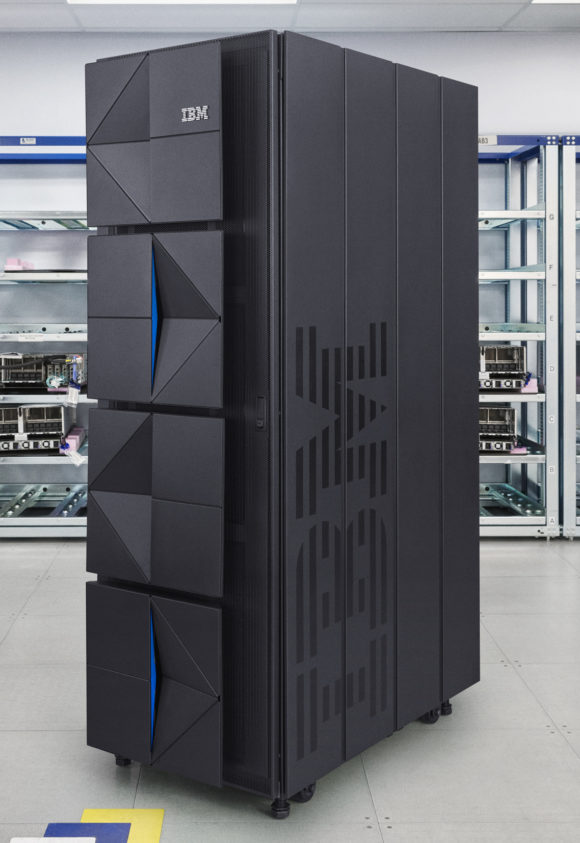
\includegraphics[width=0.40\linewidth]{bachproef//graphics/Singe_Frame_Mainframe_z16.jpg}
    \caption{Een single frame van een IBM z16 ~\autocite{Tech2023}}
    \label{fig:Een single frame van een IBM z16}
\end{figure}


Wanneer men tegenwoordig denkt aan mainframes denkt men vooral aan die van “the International Business Machines Corporation” beter bekend als IBM. IBM beheerst een gigantisch groot aandeel van de mainframe wereld wanneer het komt op beide hard- en software. In tegenstelling tot wat vaak wordt gedacht, heeft IBM de mainframe niet uitgevonden. Er waren alternatieven van andere fabrikanten, maar die zijn geleidelijk aan afgenomen, waarbij sommige bedrijven de productie zelfs volledig hebben stopgezet. Hoewel sommige bedrijven zoals Fujitsu, NEC, Unisys en Bull nog steeds eigen mainframes aanbieden, is het een afnemende markt volgens John Abbot~\autocite{DrewRobb}. Wanneer het aankomt op software heeft IBM wel meer competitie met software leveranciers zoals Broadcom en BMC al worden die producten grotendeels gebruikt op IBM’s eigen mainframes. Dit onderzoek wordt gedaan met een z16 IBM mainframe wat betekent dat vanaf dit punt verder het specifiek gaat over dat systeem tenzij anders vermeld.

\subsection{De eerste mainframes}
In dit deel van het onderzoek zal er besproken worden hoe we tot onze huidige situatie zijn geraakt wanneer het aankomt op mainframes. Want ze ondersteunen onze samenleving nu al decennia op een manier waarbij de bevolking weinig bewust contact men ze maakt. Om meer context te plaatsen op de huidige versies is het handig om eerst een blikje terug te nemen in het verleden. Het is hier niet de bedoeling dat men diepgaand een mainframe gaan onderzoeken. Een mainframe is zo breed dat dat buiten het scope van dit onderzoek valt. Er zullen dus hoogstwaarschijnlijk een aantal concepten of termen terugkomen dat iemand buiten de IT wereld niet meteen zou herkennen. Ze zijn niet belangrijk om dit onderzoek te begrijpen. Ze zou wel genoeg context moeten geven om te snappen dat een mainframe altijd blijft evolueren door nieuwe technologieen en/of concepten toe te passen. 

\subsection{z16}
De IBM z16 mainframe is in 2023 de meest recenste en geavanceerde systeem dat IBM heeft uitgebracht.Het is een aanzienlijke upgrade ten opzichte van de eerdere z15. De z16 maakt gebruik van de Telum-processor die draait op 5,2 GHz, dat is één van de snelste beschikbaar. Belangrijke verbeteringen zijn onder andere 17\% meer processor capaciteit per lade, een on-chip Accelerator for AI voor snelle AI-verwerking, en een herontworpen cache voor betere prestaties in transactionele scenario's. Het systeem behoudt een geheugencapaciteit van maximaal 40 TB met behulp van redundante array of independent memory (RAIM) technologie voor hoge beschikbaarheid. Connectiviteitsopties zijn uitgebreid en aanpasbaar aan verschillende behoeften. Door de verstaanbare behoeftes van zSystem klanten is veiligheid weer een topprioriteit, met quantum-safe mogelijkheden voor sleutelgeneratie en encryptie, evenals Pervasive Encryption voor het beveiligen van gegevens in rust en in transit. Het Security and Compliance Center is een nieuwe functie die compliance-taken vereenvoudigt. De z16 is een krachtige en veilige keuze voor bestaande IBM-mainframeklanten, met verbeteringen in prestaties, schaalbaarheid en beveiliging. Colruyt group gebruikt op dit moment deze versie van de IBM mainframes. Figuur 2.3 is een voorbeeld van een z16 mainframe met 4 frames.~\autocite{Laura2023,Steven2023}

\begin{figure}[h]
    \centering
    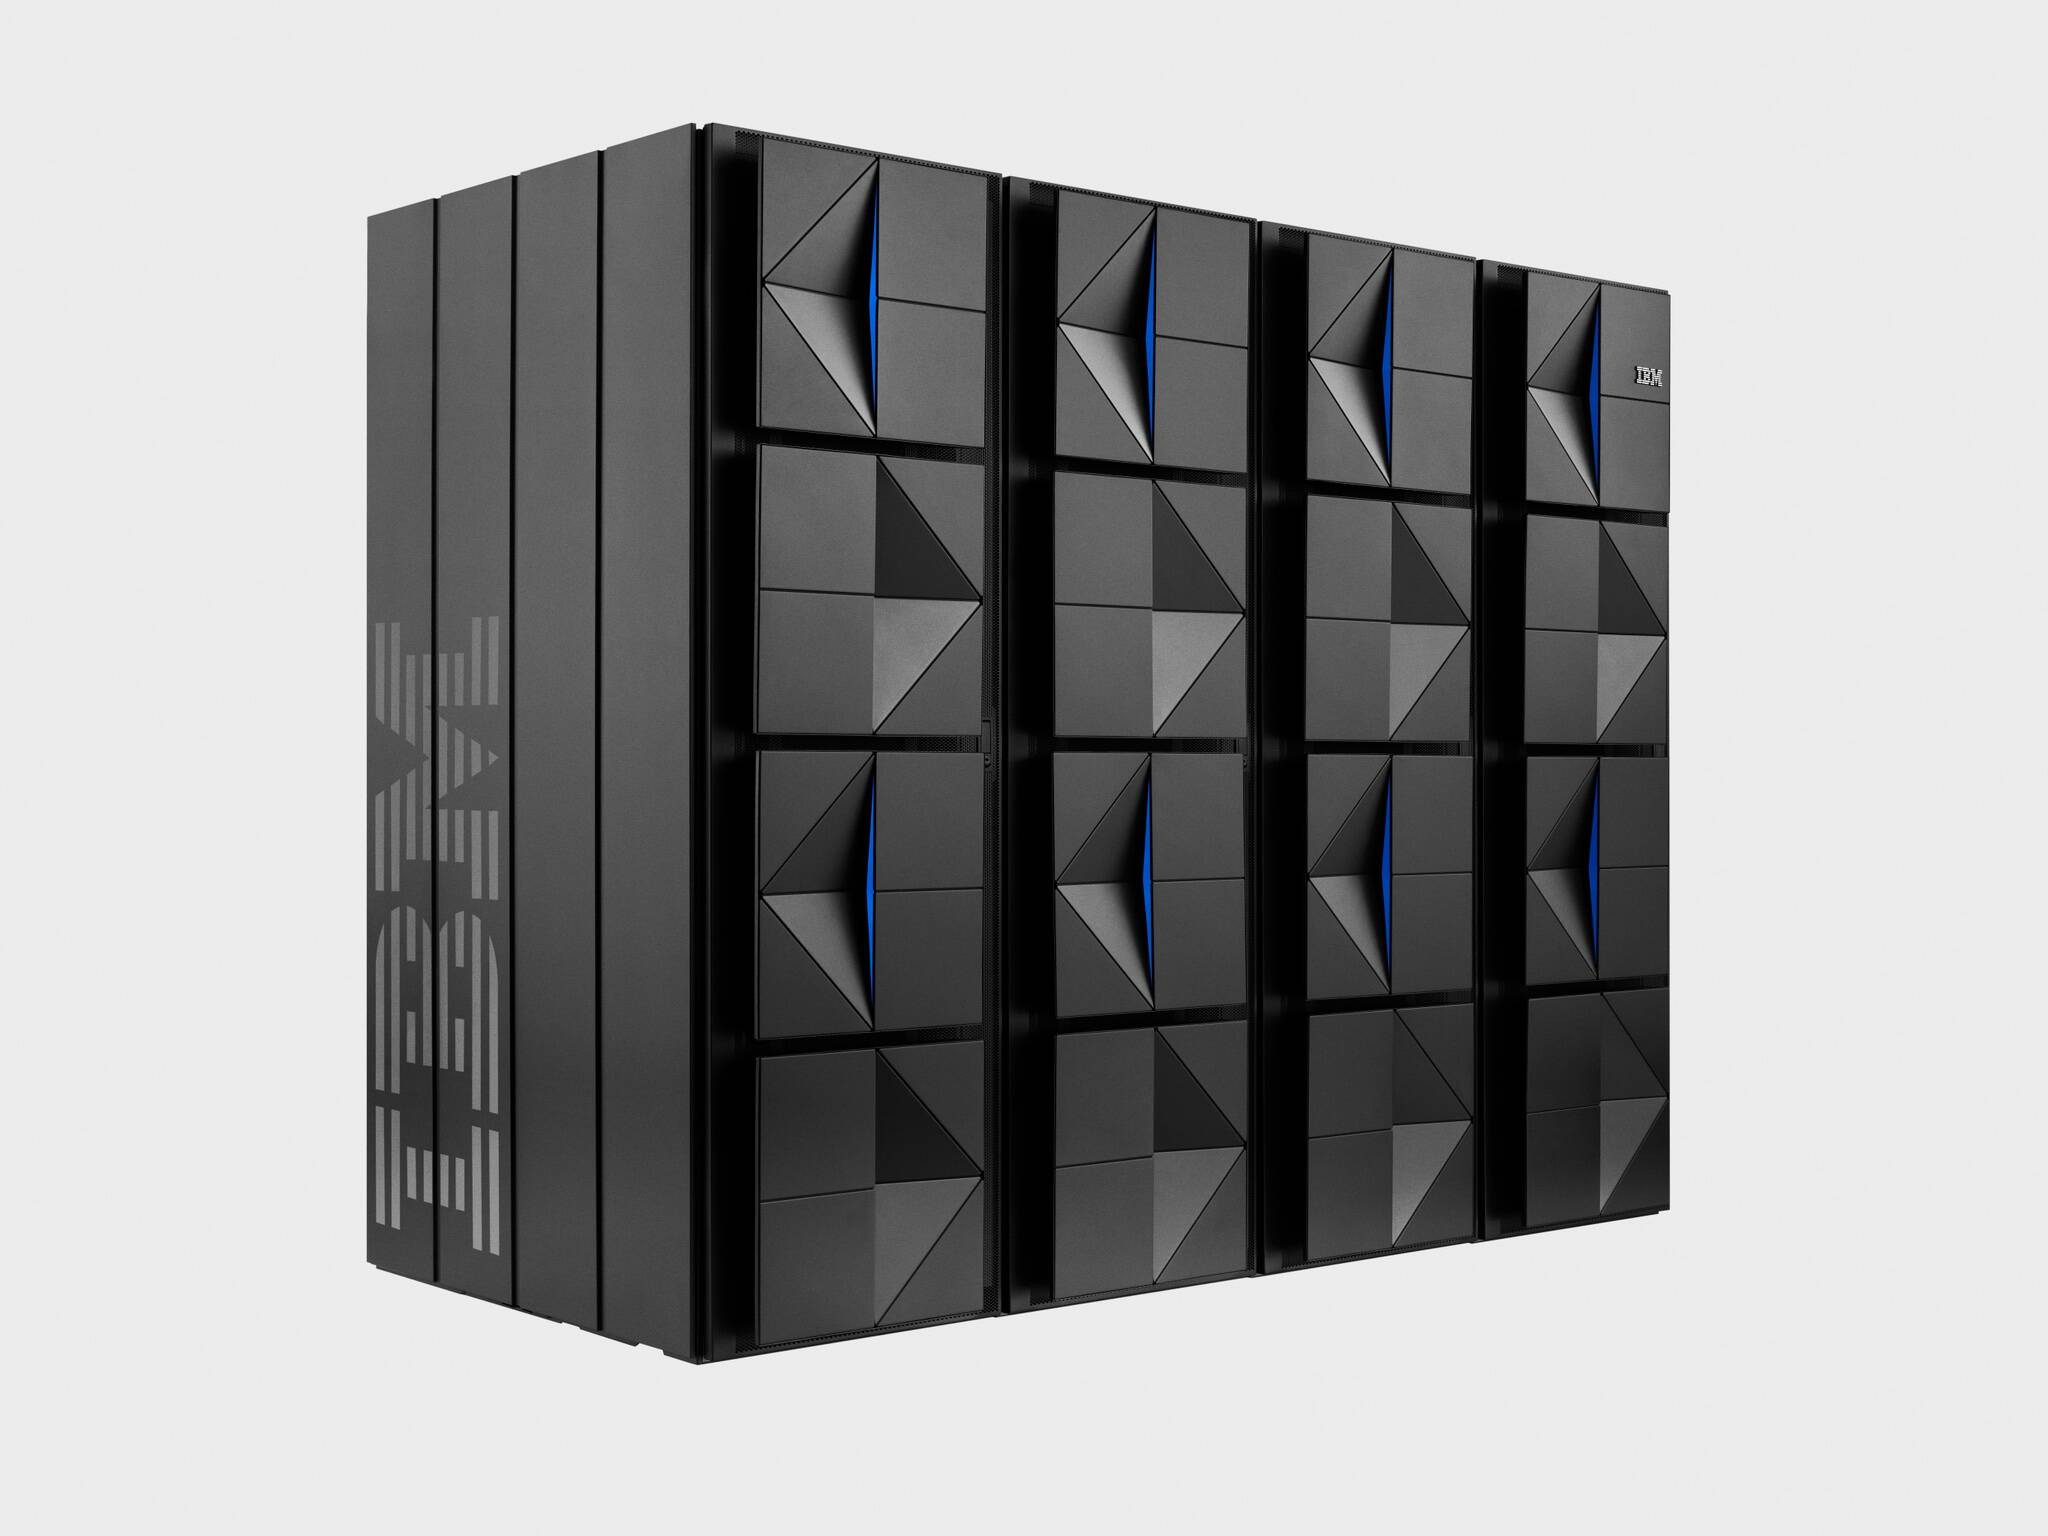
\includegraphics[width=0.5\linewidth]{bachproef//graphics/4-frame-z16.jpg}
    \caption{Een z16 met 4 frames ~\autocite{Elizabeth2022}}
    \label{fig:Een z16 met 4 frames}
\end{figure}

\subsection{Betrouwbaarheid}
Mainframes worden geprezen om hun ongeëvenaarde betrouwbaarheid. Deze betrouwbaarheid is gebaseerd op RAS-principes. RAS staat voor betrouwbaarheid (Reliability in het engels), beschikbaarheid (Availability in het engels) en Servicebaarheid. RAS zorgt voor zelfherstel van hardware en software, snelle foutcorrecties en minimale impact bij storingen. Hierdoor blijven mainframe consistent betrouwbaar en beschikbaar voor bedrijfstoepassingen. Dit doen ze op soft- en hardware niveau door zaken te voorzien zoals meerdere mogelijkheden om de mainframe van stroom te voorzien. Maar één van de belangrijkere concepten dat een mainframe toepast is het concept van een parrelel sysplex. Een parallel Sysplex is een technologie in de mainframe wereld die de betrouwbaarheid van systemen aanzienlijk verbetert. In tegenstelling tot gedistribueerde systemen, waar nodes onafhankelijk werken, stelt een parallel sysplex meerdere mainframesystemen in staat om samen te werken als een geheel. Deze samenwerkingsaanpak biedt verschillende voordelen op het gebied van betrouwbaarheid. Aangezien dat meerder mainframestystemen aanzienlijk ver van elkaar kunnen staan en toch perfect nog kunnen samenwerken. Ook worden gegevens meestal gelijk gehouden tussen machines. Dit zorgt ervoor dat als er een machine toch zou uitvallen dat een bedrijf of organisatie toch kan blijven draaien.~\autocite{FrankJDGilio,maincom,Subhasish2020}
De IBM z16 is een recente toevoeging aan deze traditie van betrouwbaarheid, met een uptime van 99.9999999\%. Dit komt neer op slechts iets meer dan 30 milliseconden downtime per server per jaar. Uit ervaring weet men dat er mainframes draaien die al jaren geen downtime hebben gehad. Deze ongeëvenaarde betrouwbaarheid maakt mainframes ideaal voor kritische toepassingen in de moderne zakelijke omgeving. Dit maakt mainframes tot een dominante keuze voor bedrijven die uptime en betrouwbaarheid in hoge belangstellen. Dus in conclusie is betrouwbaarheid één van de kernconcepten van mainframes. Zo'n kernconcept dat de "z" in z16 staat voor zero downtime. ~\autocite{IBM2023(3),JasonBloomberg,RobEnderle}

\subsection{Systeem logs}
 Wat hier nog niet besproken is geweest zijn de mainframe werknemers die er voor zorgen dat problemen opgelost of voorkomen worden. Dat is uiteraard ook een essentieël onderdeel om de mainframe standarden in betrouwbaarheid hoog te houden. Een dat de mainframe ervoor zorgt dat die werknemers hun job kunnen doen is door extensieve logs mee te geven. De log waar in dit onderzoek jet over gaat is de "SYSLOG". Systeemlogs op een mainframe zijn gegevens die worden gemaakt door het besturingsysteem en een sommige softwarecomponenten om informatie meetegeven over hun werking en enige problemen dat ze ondervinden. Ze zijn essentieel voor oplossen van problemen, onderhouden en monitoren van het systeem. Bij Colruyt Group lopen deze logs starten om zes uur 's ochtends en lopen 24 uur. Tijdens deze periode worden de logs geschreven naar een active logs om dan na 24u te worden opgeslaan en geachriveerd.
 
\subsection{JCL}
JCL,Job Control Language voluit, is een essentieel onderdeel van de mainframe en dient als communicatiemiddel tussen programma's zoals COBOL en PL/I en het besturingssysteem. Het speelt een belangrijke rol bij het uitvoeren van batch- of online verwerking. Bij batchverwerking kunnen taken bijvoorbeeld bestaan uit het verwerken van grote hoeveelheden banktransacties. Bij online verwerking daarentegen vinden real-time interacties plaats, zoals bankmedewerkers die een back-officescherm gebruiken om rekeningen te openen.Het is een soort programeertaal dat de mainframe zegt welke stappen die moet zetten om de job succesvol ui te voeren.~\autocite{tutpoint} Hier zijn stappen voor verwerken van taken met behulp van JCL:

\subsubsection{Taakinvoer}
Gebruikers dienen JCL in bij het Job Entry System (JES) van het besturingssysteem. Dit is waar alle jobs binnenkomen en voorbereid worden om uit te voeren.

\subsubsection{Taakconversie}
JCL, samen met eventuele bijbehorende procedures , worden omgezet in een interpreteerbaar formaat voor JES en wordt opgeslagen in een dataset genaamd SPOOL.

\subsubsection{Taakwachtrij}
JES bepaalt de prioriteit van taken op basis van parameters zoals CLASS en PRTY die zijn gedefinieerd in de job. Het controleert ook op fouten en steekt de job in de wachtrij als er geen fouten zijn.

\subsubsection{Taakuitvoering}
Wanneer een taak de hoogste prioriteit bereikt, wordt deze uit de wachtrij gehaald voor uitvoering. Het programma wordt uitgevoerd vanuit de SPOOL en de uitvoer wordt doorgestuurd naar de bestemming dat gespecifieerd werd in de job.

\subsubsection{opkuisen}
Na dat alles klaar is worden de toegewezen middelen vrijgegeven. De joblog wordt uit de SPOOL verwijderd dus als men die wilt oplsaan moet die naar een dataset weggeschreven worden.

\subsection{Service now}
ServiceNow is een cloudgebaseerd IT Service Management platform dat processen automatiseert. Service Now voldoet aan ITIL-richtlijnen voor servicegerichte operaties. Het maakt gebruik van machine learning voor efficiëntie en schaalbaarheid. Belangrijke functies omvatten onder andere  kosteneffectieve ondersteuning, aanpasbaarheid en gegevensbeveiliging. Binnen Colruyt Group en voor dit onderzoek wordt Service now voornamlijk gebruikt om ticketten aan te make om problemen op te lossen of producten te leveren. ~\autocite{DavidTaylor}

\section{ELK}
ELK is een groep van voormalige open-source software applicaties dat samenwerken om de ELK-stack te vormen. Er zijn drie hoofdapplicaties dat een ELK-stack maken en die zijn Elasticsearch, Logstash en Kibana. Daarbij komen soms andere applicaties zoals Beats ook bij kijken. Gemaakt en beheerd door Elastic, ELK dient om logs te analyseren en te visualiseren. Zo kunnen teams niet alleen hun logs overzichtelijk bekijken maar ook grafieken maken en vergelijken met vorige logs ofdat er iets verschilt. In dit hoofdstuk gaat er gekeken worden naar alle ELK componenten die van toepassing gaan komen tijdens dit onderzoek. Figuur 2.5 ~\autocite{DavidTaylor} geeft al een klein overzicht van hoe ELK werkt.~\autocite{DavidTaylor,DotanHorovits}


\begin{figure}[h]
    \centering
    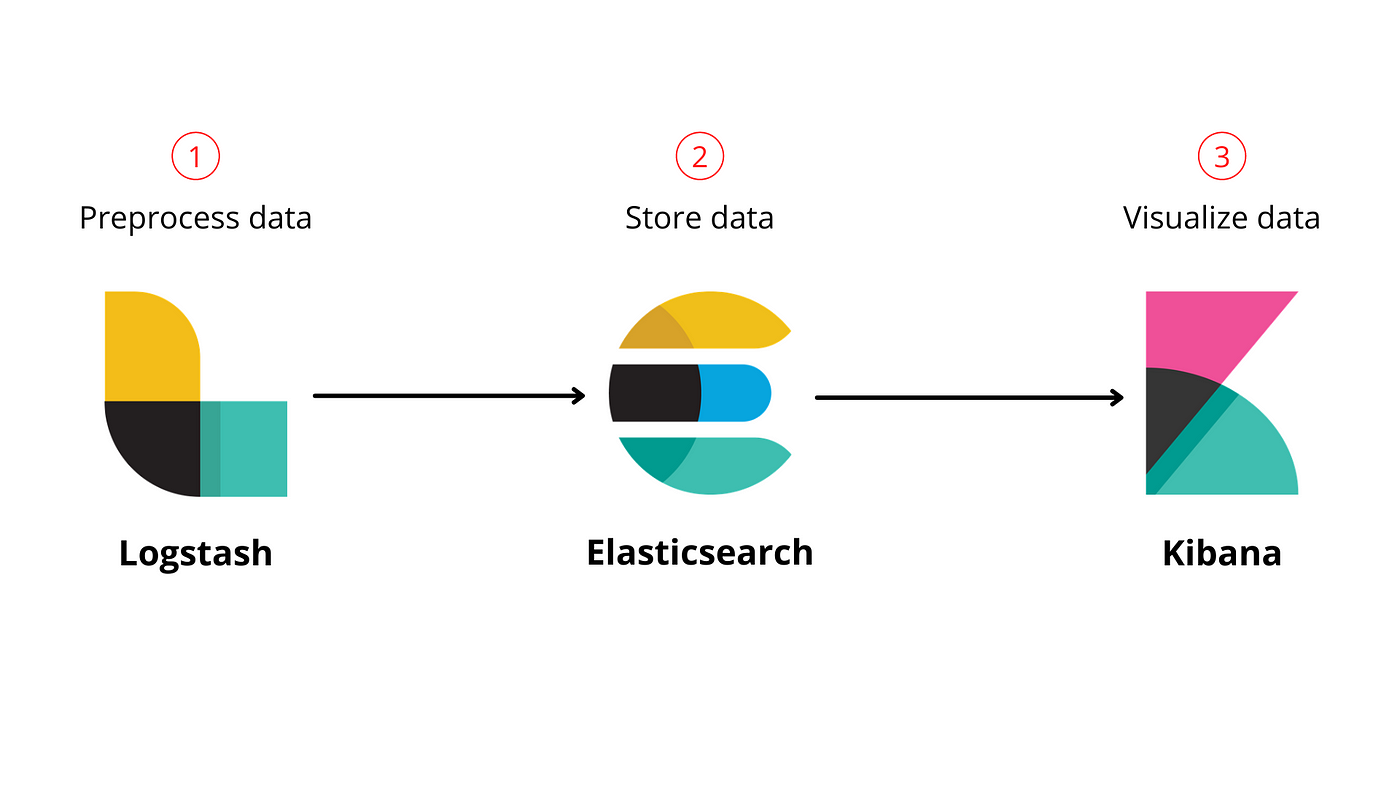
\includegraphics[width=0.5\linewidth]{bachproef//graphics/ELK_stack_essentials.png}
    \caption{Een ELK-stack met alleen de essentials ~\autocite{DavidTaylor}}
    \label{fig:Een ELK-stack met alleen de essentials}
\end{figure}

\subsection{Elastisearch}
Elasticsearch is een prominente NoSQL-database gebouwd op de krachtige Lucene-zoekmachine, bekend om zijn robuuste mogelijkheden op het gebied van gegevensopslag en -opvraging. ELk is een zoekserver is geschreven in Java en het blinkt uit in het indexeren van heterogene gegevenstypen. Elasticsearch werkt binnen een cluster, dat een verzameling nodes vertegenwoordigt die gegevens vasthouden en indexerings- en zoekmogelijkheden bieden. Nodes vertegenwoordigen individuele Elasticsearch-instanties. Gegevens zijn georganiseerd in indexen, die elk vergelijkbare documenten bevatten. Documenten worden geïndexeerd en geassocieerd met een unieke ID. Indexen kunnen worden verdeeld in shards voor distributie, en de schaalbaarheid van Elasticsearch kan worden bereikt door meer nodes aan het cluster toe te voegen. Het biedt een REST API-webinterface met JSON-uitvoer, wat integratie in verschillende toepassingen vergemakkelijkt. Elasticsearch biedt ondersteuning voor meerdere talen aan naast functies zoals volledige tekstzoekopdracht, bijna-realtime (NRT) zoekopdracht, sharding, replicatie.Een van de belangrijke voordelen is het vermogen om gegevens zonder een schema te verwerken, waardoor gebruikers gegevens record voor record kunnen manipuleren met multi-document API's. Daarnaast staat Elasticsearch bekend om zijn schaalbaarheid, zowel verticaal als horizontaal. Het ondersteunt verschillende programmeertalen dankzij de beschikbaarheid van pogammeertalen. ~\autocite{GedalBer}  

\subsection{Logstash}
Logstash is een gegevensverwerkingstool die oorspronkelijk is ontworpen voor log-analyse, maar zich heeft ontwikkeld tot een veelzijdige gegevensverwerkingstool. Het werkt als een pijplijn in 3 fases: invoer, filter en uitvoer.~\autocite{Jamie2017,JugensToit}  

\subsubsection{invoerstadium}
In het invoerstadium verzamelt Logstash gegevens uit verschillende bronnen, waaronder logbestanden, netwerkprotocollen en wachtrijen. Het kan inkomende gebeurtenissen taggen met metagegevens die verband houden met hun bron.

\subsubsection{filterstadium}
Het filterstadium in Logstash voegt aanzienlijke waarde toe door middel van filter-plugins. Deze plugins zijn verantwoordelijk voor het transformeren en verrijken van gegevens. Ze kunnen voorwaardelijke logica toepassen op basis van eigenschappen van gebeurtenissen, velden extracten en bewerkingen uitvoeren zoals het parseren van tijdstempels en het omzetten van gegevenstypen. Het correct rangschikken van deze filter-plugins is van cruciaal belang om een efficiënte gegevensverwerking te verzekeren.

\subsubsection{uitvoerstadium}
Het uitvoerstadium handelt de levering van verwerkte gebeurtenissen naar verschillende bestemmingen af, zoals databases, wachtrijen, API's en meer. Logstash ondersteunt meerdere uitvoerkanalen voor een enkele gebeurtenis, waardoor het zeer aanpasbaar is voor verschillende use-cases. Logstash biedt ook codecs, die bepalen hoe gegevens worden geserializeerd of gedeserialiseerd. Codecs zijn bijzonder nuttig voor het verwerken van gestructureerde gegevensformaten zoals JSON of meerregelige logvermeldingen.Wat betreft architectuur kan Logstash worden ingezet in verschillende configuraties, van single-server configuraties tot complexe gedistribueerde infrastructuren. De keuze voor de architectuur hangt af van de schaal en de vereisten voor log-verwerking.Logstash is een fundamenteel onderdeel in Extract-Transform-Load (ETL) pijplijnen gewirden, waarbij gegevens effectief worden verwerkt uit diverse bronnen en formaten.

\subsection{Kibana}
De K van ELK staat voor Kibana het programma dat verantwoordelijk is voor visualisatie en analysatie. Het interface dat toegang geeft aan de visualisatie mogelijkheden van Kibana is in dashboard formaat. Een ELK-dashboard bestaat uit verschillende panelen dat de gebruiker zelf kan instellen.~\autocite{Elatic(1)} Figuur 2.5 is een voorbeeld van een dashboard. Een paneel kan uitvolgende soorten bestaan:

\begin{itemize}
    \item Editors
        Editors is een collectie van panelen die onderandere dienen om grafieken weer te geven. Voorbeelden zijn tabbellen, heatmap en treemaps. 
    \item Maps
        Het doel van deze panelen is om geografische kaarten te maken van de beschikbare gegevens.

    \item Anomaly swim lane
        Met deze paneel kan een gebruiker naar de resulaten van de anomaly detection kijken. Meer over Anomaly detection later.
        
    \item Anomaly chart
       Deze paneel geeft de gebruiker de mogelijkheid om een grafiek van anomalies te zien.
        
    \item Log stream
        Deze paneel dient om de huidige logs te zien dat ELK binnenkrijgt.

    \item Tools
        Deze paneel geeft de mogelijk om interactieve filter mogelijkheden te maken. Een voorbeeld hiervan is time slider dat u de optie geeft om te filteren op een start en eind tijd.

    \item Text
        Met deze paneel kan u makkelijk tekst toevoegen aan uw dashboard. Dit kan handig zijn om documentatie of instructies te schrijven.

    \item Image
        Om uw dashboard te kunnen personaliseren is er ook een mogelijkheid om foto's of logo's op uw dashboard te zetten. Dit kan met foto's van op uw computer of externe links.
\end{itemize}


\begin{figure}[h]
    \centering
    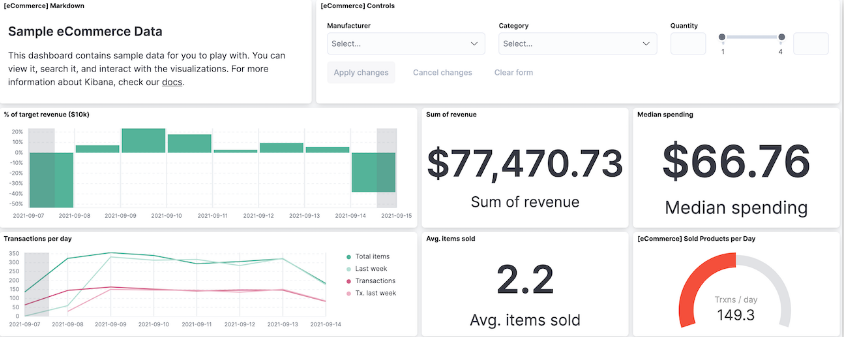
\includegraphics[width=0.75\linewidth]{bachproef//graphics/Voorbeeld_Dashboard.png}
    \caption{Een voorbeeld van een ELK dashboard ~\autocite{Eleanor2023}}
    \label{fig:een voorbeeld van een ELK dashboard}
\end{figure}

\subsection{Beats}
Zoals eerder vemeldt is geweest kunnen er naast de drie ELK-programma's andere programma's ELK ondersteunen. Onder deze programma's is het Beats-ecosysteem bijzonder opmerkelijk en de meest voorkomende. Beats zijn in wezen lichtgewicht agenten die zijn ontworpen voor specifieke taken voor gegevensverzameling en die verzamelde gegevens overdragen naar Elasticsearch. Zulke applicaties worden wel 'data-shippers' genoemd. Wanneer men Beats toevoegt aan ELK spreekt men dan meestal van een Elastic-stack. De sleutel tot de veelzijdigheid van Beats ligt in het libbeat-framework. Dit framework vereenvoudigt het maken van aangepaste gegevens verzamelingsagents, waardoor het haalbaar is om Beats aan te passen aan verschillende soorten gegevens. Als gevolg daaraan blijft het Beats-ecosysteem snel groeien. Op dit moment zijn er zes officiële Beats ontwikkeld door Elastic. Deze Beats zijn open source en vallen onder de Apache-licentie. Samen pakken ze het veelvoorkomende probleem aan van het efficiënt verzamelen van gegevens en het doorsturen ervan naar Elasticsearch.~\autocite{objectrocket}  

\subsubsection{Filebeat}
eerst ontworpen voor het lezen van bestanden vanuit het systeem, is Filebeat met name handig voor het verwerken van systeem- en toepassingslogbestanden. Het stroomlijnt de centralisatie van logs door logs van verschillende servers en Virtuele machines te lezen en door te sturen naar een centrale Logstash- of Elasticsearch-instantie. Daarnaast vereenvoudigt Filebeat de configuratie met vooraf gebouwde modules voor veelvoorkomende logbestandsindelingen.

\subsubsection{Metricbeat}
Metricbeat specialiseert zich in het verzamelen van metingen van servers en systemen, wat ideaal is voor het monitoren van systeem- en service-statistieken. Net als Filebeat bevat Metricbeat modules voor verschillende besturingssystemen en toepassingen, wat zorgt voor minimale impact op systeemprestaties.

\subsubsection{Packetbeat}
Packetbeat fungeert als een lichtgewicht netwerkpacketanalyzer en bewaakt continu netwerkprotocollen om inzicht te bieden in netwerklatentie, fouten, responstijden en meer. Het ondersteunt meerdere toepassingslaagprotocollen.

\subsubsection{Winlogbeat}
Speciaal ontworpen voor Windows-omgevingen, levert Winlogbeat live streams van Windows-logboek gebeurtenissen. Het bewaakt verschillende gebeurtenissen, zoals aanmeldingen, USB-apparaatgebruik en software-installaties, en stuurt deze gegevens door naar Elasticsearch voor beveiligingsmonitoring.

\subsubsection{Auditbeat}
Voor Linux-platforms voert Auditbeat een gelijkiaardige functie uit door gebruikers- en procesactiviteit over het systeem te bewaken. Audit-gegevens worden in realtime naar Elasticsearch verzonden voor beveiligingsmonitoring.

\subsubsection{Heartbeat}
Heartbeat kan systemen pingen om te zien of ze nog operationeel zijn. Deze info wordt dan naar ELK gestuurd. Het ondersteunt meerdere protocollen en functies, waaronder TLS, verificatie en proxies, en lost efficiënt DNS op om hosts achter load-balanced servers te monitoren.


\begin{figure}[h]
    \centering
    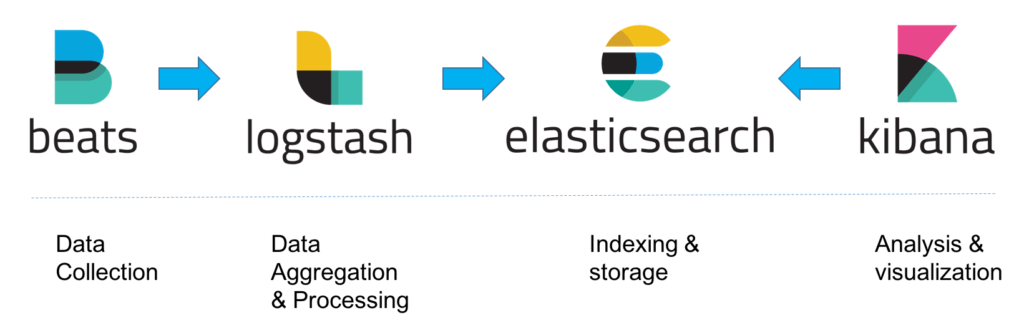
\includegraphics[width=0.5\linewidth]{elk_stack_beats.png}
    \caption{Een ELK-stack met beats ~\autocite{DavidTaylor}}
    \label{fig:Een ELK-stack met beats}
\end{figure}

\subsection{Anomaly detection}
Ook staan we even stil bij deviatie detectie functies dat Elastic aanbiedt. Dat is een live hulpmiddel binnen de Elastic Stack dat bedoeld is om afwijkingen in tijdreeksgegevens te identificeren. Het leert autonoom de normale patronen en trends in de gegevens, vermindert valse alarmen en vereenvoudigt de analyse van de onderliggende oorzaken. Deze functie zou erg van pas komen voor MFPOSS. Belangrijke onderdelen zijn:
\begin{itemize}
    \item Jobbeheer voor het maken en beheren van taken voor deviatie detectie.
    \item Kalenderbeheer voor aangepaste regels.
    \item Visualisatietools zoals de deviatie-verkenner en de Weergave van enkele metrieken.
    \item Handmatige of automatische annotaties toevoegen aan afwijkingen voor context.*
    \item Het Jobbeheerpaneel houdt een uitgebreide lijst van annotaties bij voor elke taak.
\end{itemize}


Al deze onderdelen helpen bij het volgen van afwijkingen en het verbeteren van de operationele werkingen.
*Automatische annotaties worden toegevoegd voor situaties zoals ontbrekende gegevens. ~\autocite{Elatic(2)} 

\section{DataDog}

\section{Grafana}

\section{Linux}

\subsection{Linux Server}

\subsection{RedHat}

\subsection{FTP}
%%=============================================================================
%% Methodologie
%%=============================================================================

\chapter{\IfLanguageName{dutch}{Methodologie}{Methodology}}%
\label{ch:methodologie}

In dit hoofdstuk stellen we de verwachtingen van MFPOSS vast. Dit doen we zodat het prototype geëvalueerd kan worden zodra het is voltooid. Dit wordt het best gedaan aan de hand van de MoSCoW-methode. Deze methode houdt in dat van tevoren wordt bepaald wat MFPOSS wil van het product, en deze criteria worden verdeeld in de volgende categorieën:

\begin{itemize}
    \item Must have
    \item Should have
    \item Could have
    \item Won't have
\end{itemize}

\section{MoSCoW}

\subsection{Must have}
Voor MFPOSS is het belangrijk dat er eenvoudig te zien is welke berichten vaak voorkomen en welke zelden voorkomen.

\subsection{Should have}
Het is ook de taak van ELK om het leven voor MFPOSS makkelijker te maken zonder dat er te veel extra werk aan besteed moet worden. Het moet dus eenvoudig zijn om elementen aan het dashboard toe te voegen zonder veel programmeerwerk. Het is ook belangrijk dat MFPOSS afwijkingen kan detecteren. Deviatiedetectie kan hierbij goed helpen.

\subsection{Could Have}
Het zou interessant zijn om te onderzoeken of er automatisch meldingen naar MFPOSS kunnen worden gestuurd als ELK iets ongewoons opmerkt.

\subsection{Won't Have}
Een complexe implementatie waaruit te weinig informatie kan worden gehaald. Daarnaast mag het niet te veel extra werk vergen om zaken aan te passen of toe te voegen.

Nadat een prototype is opgesteld voor elke analyser, zal worden beoordeeld of het voldoet aan de vooraf vastgestelde MoSCoW-criteria. Als het prototype niet ten minste aan de "Must have" en "Won't have" criteria voldoet, betekent dit dat het voor MFPOSS niet voldoende is om verder mee te werken. Alle analysers dat overblijven gaan worden vergeleken met elkaar wanneer het aankomt op gemak van gebruik, stijl, prijs en effeicientie.

\Section{Linux}
Een mainframe heeft zoals eerder besproken limitaties dat boven komen doordat het een niche platform is. Dit zou voor problemen kunnen zorgen wanneer het aankomt op support. Gelukkig voor mainframe teams kan de mainframe een Linux server draaien waarop er vandaag de dag meer support is voor de log analysers. Op deze methode omzeilen we niet alleen de limitaties van een mainframe maar geraken we ook terecht in een situatie waar traditionele bedrijven zich ook meestal vinden aangezien een groot deel daarvan Linux servers gebruiken of allesinds toegang kunnen vergrijgen tot één. Ook is dit handig voor bedrijven met meerdere mainframe teams aangezien dat logs zich op verschillende plaatsen kunnen vinden en het niet altijd even eenvoudig is om ze rechstreeks naar de analyser te sturen. Maar als er een Linux server bestaat kan dit dienen als soor landing zone voor alle teams en kan er van hier uit een reproduceerbare methode gevonden worden om alle logs te versturen. Om dit te doen moet er natuurlijk eerst een Linux server oopgesteld worden. 

TO DO: Linux server op mainframe opstellen?
\subsection{Linux op mainframe}

\subsection{Versturen van data}
Nu moet alleen de link gemaakt kunnen worden van de mainframe naar de linux server. Dit gaat gebeuren aan de hand van een JCL job. Die job gaat ervoor zorgen da we de logbestanden kunnen FTPen naar de Linux server en ze meteen in de goeie directory kunnen steken.

\begin{figure}[h]
    \centering
    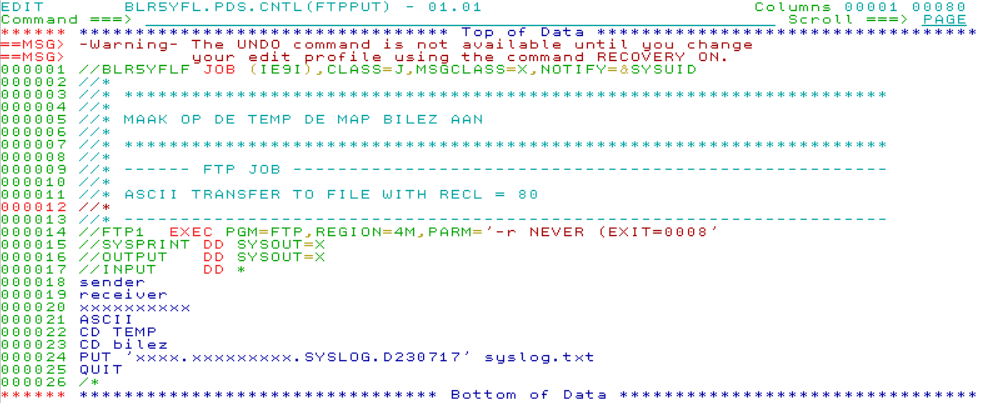
\includegraphics[width=1\linewidth]{bachproef//graphics/FTP JCL.png}
    \caption{Een voorbeeld van hoe een JCL-bestand voor FTP eruit kan zien}
    \label{fig:Een voorbeeld van hoe een JCL-bestand voor FTP eruit kan zien}
\end{figure}

Figuur 4.4 is een voorbeeld van een JCL-taak die bedoeld is om een bestand via FTP naar een bepaalde locatie te verzenden. Regel één is een standaard JCL-regel, waarbij de enige relevante variabelen de naam van de taak en het projectnummer zijn. Er zijn meer opties, maar die vallen buiten de reikwijdte van dit onderzoek. Regels twee tot en met dertien zijn opmerkingen. Regel veertien geeft aan dat dit een FTP-taak is. Vanaf regel achttien beginnen de variabelen en commando's om het bestand succesvol over te brengen:

\begin{itemize}
    \item lijn 18: De naam van het systeem dat het bestand verstuurt.
    \item lijn 19: De naam van het systeem dat het bestand ontvangt.
    \item lijn 20: Het wachtwoord van het ontvangende systeem.
    \item lijn 21: Het formaat van de inhoud van het bestand; voor dit onderzoek zou hoogstwaarschijnlijk voor ASCII worden gekozen.
    \item lijnen 22-23: Dit zijn commando's om naar de juiste directory te navigeren.
    \item lijn 24: Plaats het bestand van waar het is opgeslagen op het systeem dat verzendt naar de huidige locatie op het ontvangende systeem. Dit wordt gevolgd door de naam die het bestand moet hebben.
    \item lijn 25: Een commando om de FTP-sessie te beëindigen.
\end{itemize}

Een aangepaste versie van deze JCL-taak zou dan zijn verstrekt aan een team dat verantwoordelijk is voor de planning van taken om deze periodiek uit te voeren.
\chapter{\IfLanguageName{dutch}{Opstellen ELK}{Opstellen ELK}}%
\label{ch:Opstellen ELK}
In dit hoofdstuk zal worden gekeken hoe er toegang tot ELK kan worden verleend aan MFPOSS en welke voorbereidingen we hiervoor moeten treffen. Het is niet de bedoeling ELK op de mainframe te installeren, aangezien Colruyt Group Services al ELK buiten de mainframe gebruikt en een team heeft dat het beheert.

\section{Opstellen ELK voor MFPOSS}
Het doel van dit onderzoek is om een prototype van een ELK-dashboard te kunnen leveren aan MFPOSS om te beoordelen of het aan de MoSCoW-eisen voldoet. Om dit te bereiken, moet eerst een contactpersoon worden gevonden bij ELK om te verkennen welke mogelijkheden er zijn om onze data naar ELK te sturen. Het eerste contact met ELK was met Anusha, zij is een medewerker in het OPMONTOOLS-team dat ELK beheert. Vanaf dit punt zullen ze worden aangeduid als het ELK-team. Voordat we doorgaan met het onderzoek, is het belangrijk om te weten of er mogelijkheden zijn om de SYSLOGS naar het ELK-team te sturen. Na een vergadering met Dieter en daarna met Anusha is snel geconcludeerd dat we de gegevens periodiek over TCP/IP kunnen verzenden. Er zijn vermoedens dat Filebeat hiervoor misschien ook kan worden gebruikt, indien nodig. Het besluit om gegevens te verzenden, moet worden genomen voordat ELK wordt opgezet, om onnodig werk te voorkomen. Zodra is besloten dat er een grote kans is om de logs succesvol naar ELK te kunnen sturen, is er een aanvraag ingediend om toegang te krijgen tot ELK. Deze aanvraag is ingediend via ServiceNow. Een verantwoordelijke van het ELK-team zal die aanvraag oppakken en ons verder helpen. Anusha heeft ook gemeld dat als er geen problemen zijn, we binnen tien dagen een integratie kunnen verwachten.


\begin{figure}[h]
    \centering
    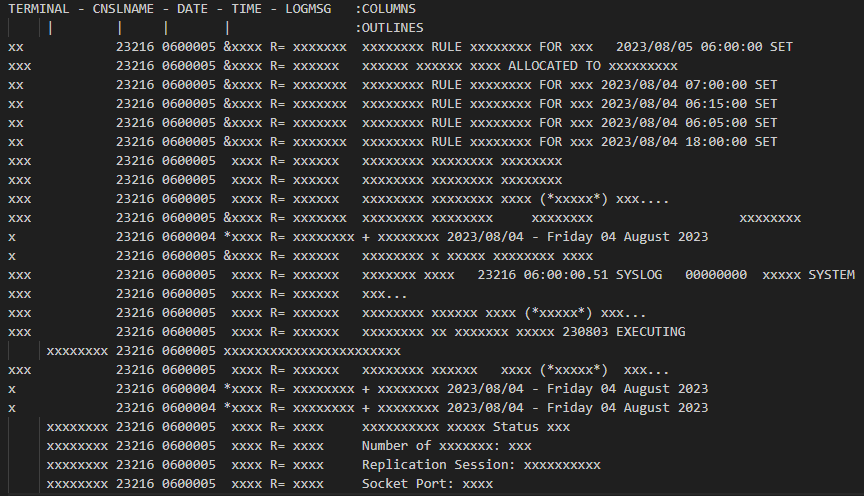
\includegraphics[width=1\linewidth]{bachproef/graphics/Voorbeeld_Syslog.png}
    \caption{Een voorbeeld van een SYSLOG met placeholdergegevens}
    \label{fig:Een voorbeeld van een SYSLOG met placeholdergegevens}
\end{figure}

Dit tekstbestand is per e-mail naar de verantwoordelijken voor de ELK-integratie van MFPOSS gestuurd. Daarbij is ook uitgelegd hoe het voorbeeld is opgebouwd. De eerste regel bevat alle kolomnamen. Daaronder staan regels die het begin van een nieuwe kolom vertegenwoordigen. Vanaf regel drie begint de log zelf. Nu de verantwoordelijken het bestand hebben ontvangen, kunnen ze doorgaan met het opzetten van ELK. Ze hadden ook details nodig over enkele velden, zoals hoe de datum is opgebouwd uit twee tekens voor het jaar en drie tekens voor de dag van het jaar.

\subsection{Mockup}
Nadat een voorbeeld is verzonden, beschikken de verantwoordelijken over alle benodigde informatie om de ELK-integratie voor MFPOSS uit te voeren. Er volgden ook nog enkele vergaderingen waarin het ELK-team details wilde bespreken en bevestigen. Nu de ELK-integratie volop in gang is, kunnen we gelijktijdig beginnen met het ontwerpen van een mock-up voor het dashboard. Dit is het onderwerp van dit hoofdstuk. Op basis van de verwachtingen kunnen we concluderen dat MFPOSS een dashboard nodig heeft waarmee de volgende taken kunnen worden uitgevoerd via panelen:

1. Het bekijken van bepaalde logs.
2. Het detecteren van afwijkingen om te zien of er opvallende gebeurtenissen zijn opgetreden.
3. Mogelijk is er behoefte aan een plek voor documentatie.
4. Een grafiek met interessante gegevens, zoals de meest voorkomende logboekmelding.

\subsubsection{Probleem één}
Tijdens een van de vergaderingen met het ELK-team werd gevraagd naar afwijkingdetectie en wat de mogelijkheden waren om dit in een dashboard te integreren. Het blijkt dat de ELK-stack van Colruyt Group op dat moment nog geen afwijkingdetectie ondersteunt. Dit is een tekortkoming voor MFPOSS, maar het is geen reden om het onderzoek vroegtijdig te stoppen. Met deze nieuwe informatie kunnen we punt twee schrappen. Dit geeft ons ruimte om een andere grafiek toe te voegen.

\begin{figure}[h]
    \centering
    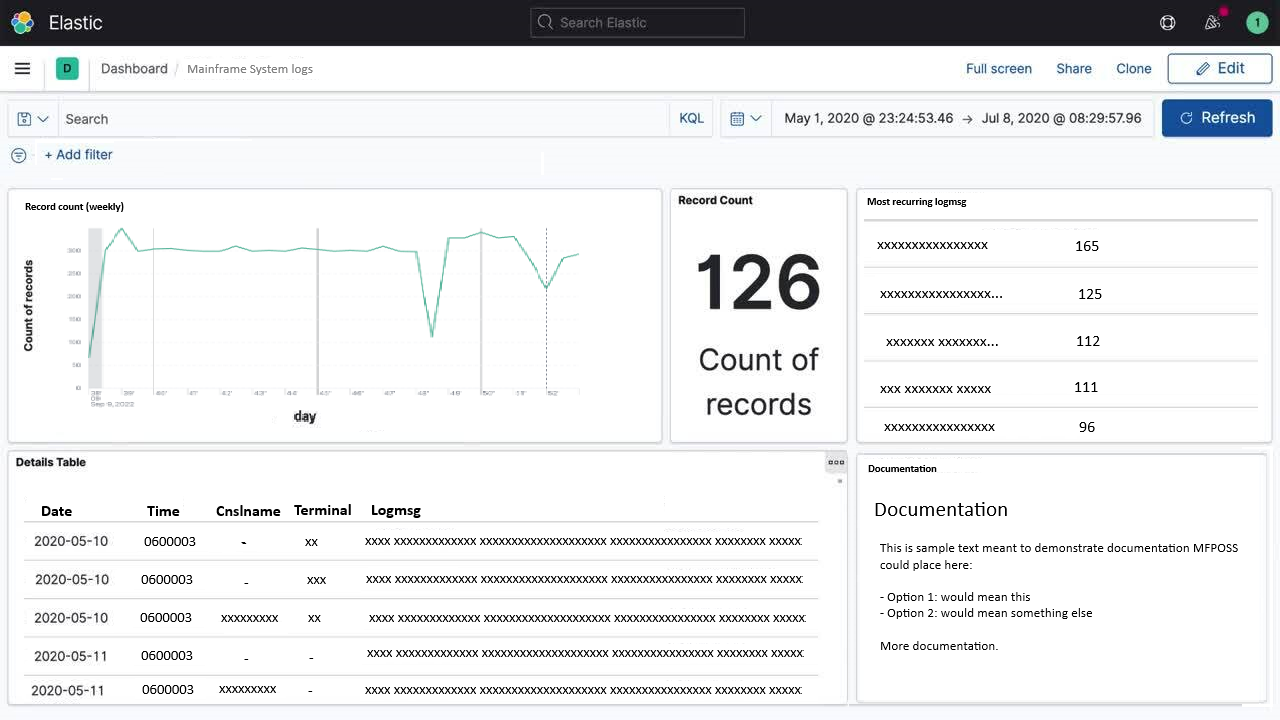
\includegraphics[width=1\linewidth]{bachproef//graphics/Dashboard_mockup.png}
    \caption{De mock-up voor het ELK-dashboard van MFPOSS}
    \label{fig: De mock-up voor het ELK-dashboard van MFPOSS}
\end{figure}

Figuur 4.3 is een mock-up van een dashboard dat mogelijk wordt verwacht. Het dashboard bestaat naast de Elastic-header uit vijf panelen. Er wordt hier natuurlijk gewerkt met fictieve gegevens die zo goed mogelijk echte gegevens proberen te representeren. Laten we kort de panelen bespreken. Het paneel op de eerste rij is een paneel met een lijngrafiek. Dit dient om te laten zien hoeveel regels de logs bevatten gedurende de afgelopen zeven dagen. Daarnaast is er een kleiner paneel dat snel het aantal regels weergeeft dat vandaag is ontvangen. Dit is handig om gemakkelijker te vergelijken met voorgaande dagen op de grafiek. Paneel drie is een lijst met de meest voorkomende regels. Een ervaren medewerker zou hier hopelijk al afwijkingen kunnen opmerken, aangezien afwijkingdetectie niet wordt gebruikt binnen Colruyt Group. Het tweede rij aan panelen bevat er twee: links de meest recente logs die ELK heeft ontvangen, en rechts een kader dat dient voor documentatie, tips of notities. Dit dashboard bevat al een groot deel van wat MFPOSS snel wil zien. Maar als men dieper in de gegevens wil kijken, is er ook de mogelijkheid om velden te doorzoeken en te visualiseren met behulp van de zoekbalk bovenaan.



\chapter{\IfLanguageName{dutch}{Opstellen Dashboard}{Opstellen Dashboard}}%
\label{ch:Opstellen Dashboard}

\section{Kibana}

Het heeft veel langer geduurd dan verwacht om de ELK-integratie op te zetten. Het ELK-team had niet genoeg tijd vanwege ander werk dat ze moesten verrichten. Dit betekent dat er voor het onderzoek niet genoeg tijd zal zijn om het dashboard tijdig op te zetten en te analyseren. Op het moment van schrijven zijn nog steeds de juiste machtigingen gegeven om dashboards aan te maken. Het onderzoek zal nu doorgaan met wat we hebben en zal theoretisch concluderen of een dashboard de moeite waard is voor MFPOSS. Dit neemt een groot stuk uit het onderzoek maar geeft ons nog wel genoeg om tot een conclusie te komen.

\subsection{Toegang tot Kibana}
De huidige situatie is dat er toegang is verleend aan de testomgeving voor Kibana, via een link die door het ELK-team is verstrekt. Hier kan worden gezocht naar "Mainframe systemlogs" om enkele van onze logs te bekijken die handmatig zijn geüpload. Er waren enkele problemen met toegangsrechten en permissies met onze gebruikelijke accounts. Om dit probleem op te lossen, heeft het ELK-team een account gemaakt dat aan de juiste voorwaarden voldoet. Met deze gegevens kunnen we al een aantal zaken testen die op het dashboard kunnen verschijnen.

\subsection{Kibana Discover}
In dit hoofdstuk gaan we onderzoeken of we met de testlogs kunnen zien of het theoretisch mogelijk is om een dashboard te maken dat geschikt is voor MFPOSS. Dit doen we door de gegevens apart te visualiseren en de panelen van de mockup na te bootsen.

\subsubsection{Probleem twee}
Naast het eerder besproken probleem met de permissies was er ook een probleem met de logs die we hadden geüpload. De volledige logboekmelding, inclusief datum, tijd, cnslname en terminal, bevond zich in hetzelfde veld, terwijl alle andere velden leeg waren. Dit probleem kon worden opgelost door de logs handmatig opnieuw te uploaden. De onjuiste gegevens staan nog steeds in ELK, maar kunnen eenvoudig worden vermeden. Daarnaast zijn de datum- en tijdvelden niet zoals verwacht, maar gelukkig kunnen we er nog steeds mee werken. Deze moeten later worden aangepast door een lid van het ELK-team.

\subsubsection{Paneel één}
Het eerste paneel op de mockup had tot doel een weergave te geven van het aantal keren dat elk type terminal in de laatste 7 dagen voorkwam. Voor dit specifieke paneel was er niet genoeg gegevens beschikbaar over meerdere dagen. Daarom hebben we ervoor gekozen om het aantal keren dat een terminal voorkwam in een kolomgrafiek weer te geven. Dit had ook een lijngrafiek kunnen zijn met het aantal records in de laatste zeven dagen. Dit paneel wordt als succesvol beschouwd.

\begin{figure}[h]
    \centering
    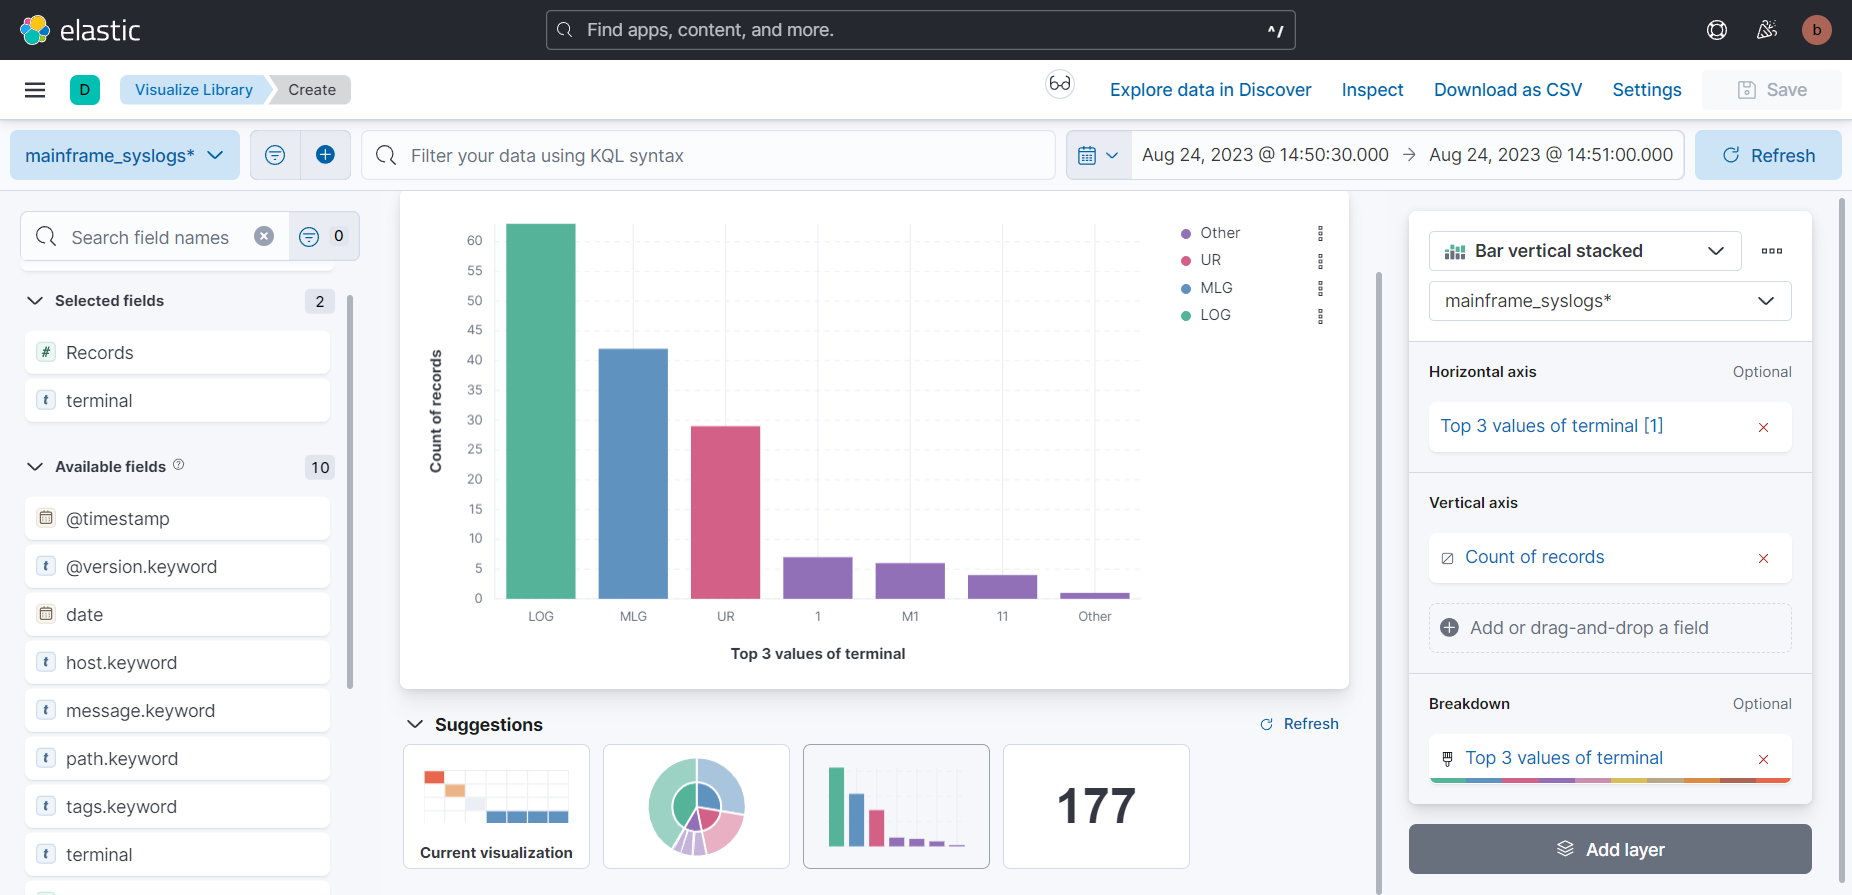
\includegraphics[width=0.50\linewidth]{bachproef//graphics/kibana_bar_chart.png}
    \caption{Een kolomgrafiek van het aantal keren dat een terminal voorkwam}
    \label{fig:Een kolomgrafiek van het aantal keren dat een terminal voorkwam}
\end{figure}

\subsubsection{Paneel twee}
Paneel twee van de mockup was een optelling van alle rijen in het meest recente log. Dit is succesvol gerepliceerd in Kibana. Het kan worden gezien in figuur 5.2. Er zijn ook andere interessante statistieken die MFPOSS mogelijk kan gebruiken.

\begin{figure}[h]
    \centering
    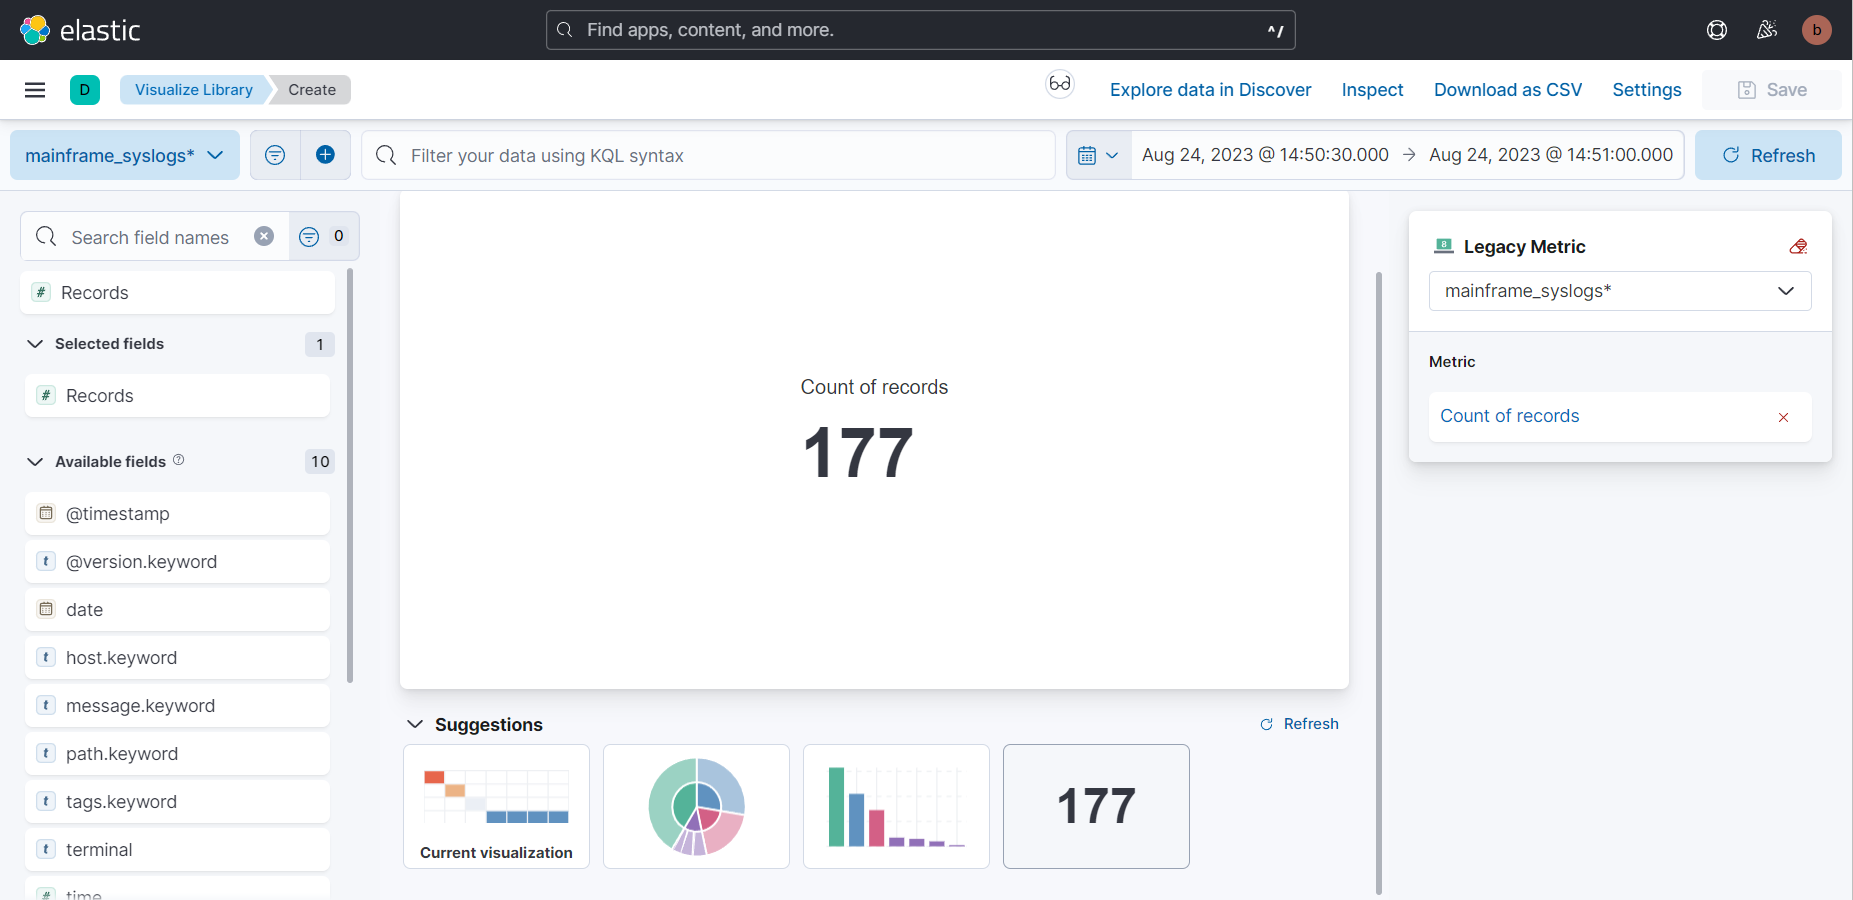
\includegraphics[width=0.50\linewidth]{bachproef//graphics/kibana_record_panel.png}
    \caption{De replicatie van paneel twee}
    \label{fig:De replicatie van paneel twee}
\end{figure}

\subsubsection{Paneel drie}
Paneel drie zou normaal gesproken deviatiedetectie bevatten, maar aangezien dit niet wordt gebruikt in Colruyt, is besloten om van paneel drie een weergave te maken van het meest voorkomende logbericht. Dit kan met minimale extra inspanning worden gedaan. Aangezien het enigszins vergelijkbaar is met paneel één, bespreken we hier ook kort de mogelijkheden om snel statistieken te bekijken. Dit kan worden gedaan door te hoveren over een veld of door de veldstatistieken tab te gebruiken. Een ervaren MFPOSS-medewerker zou hier in principe de mogelijkheid hebben om te beoordelen of er een probleem of afwijking is. De volgende afbeeldingen laten zien hoe deze statistieken eruit zien.

\begin{figure}[h]
    \centering
    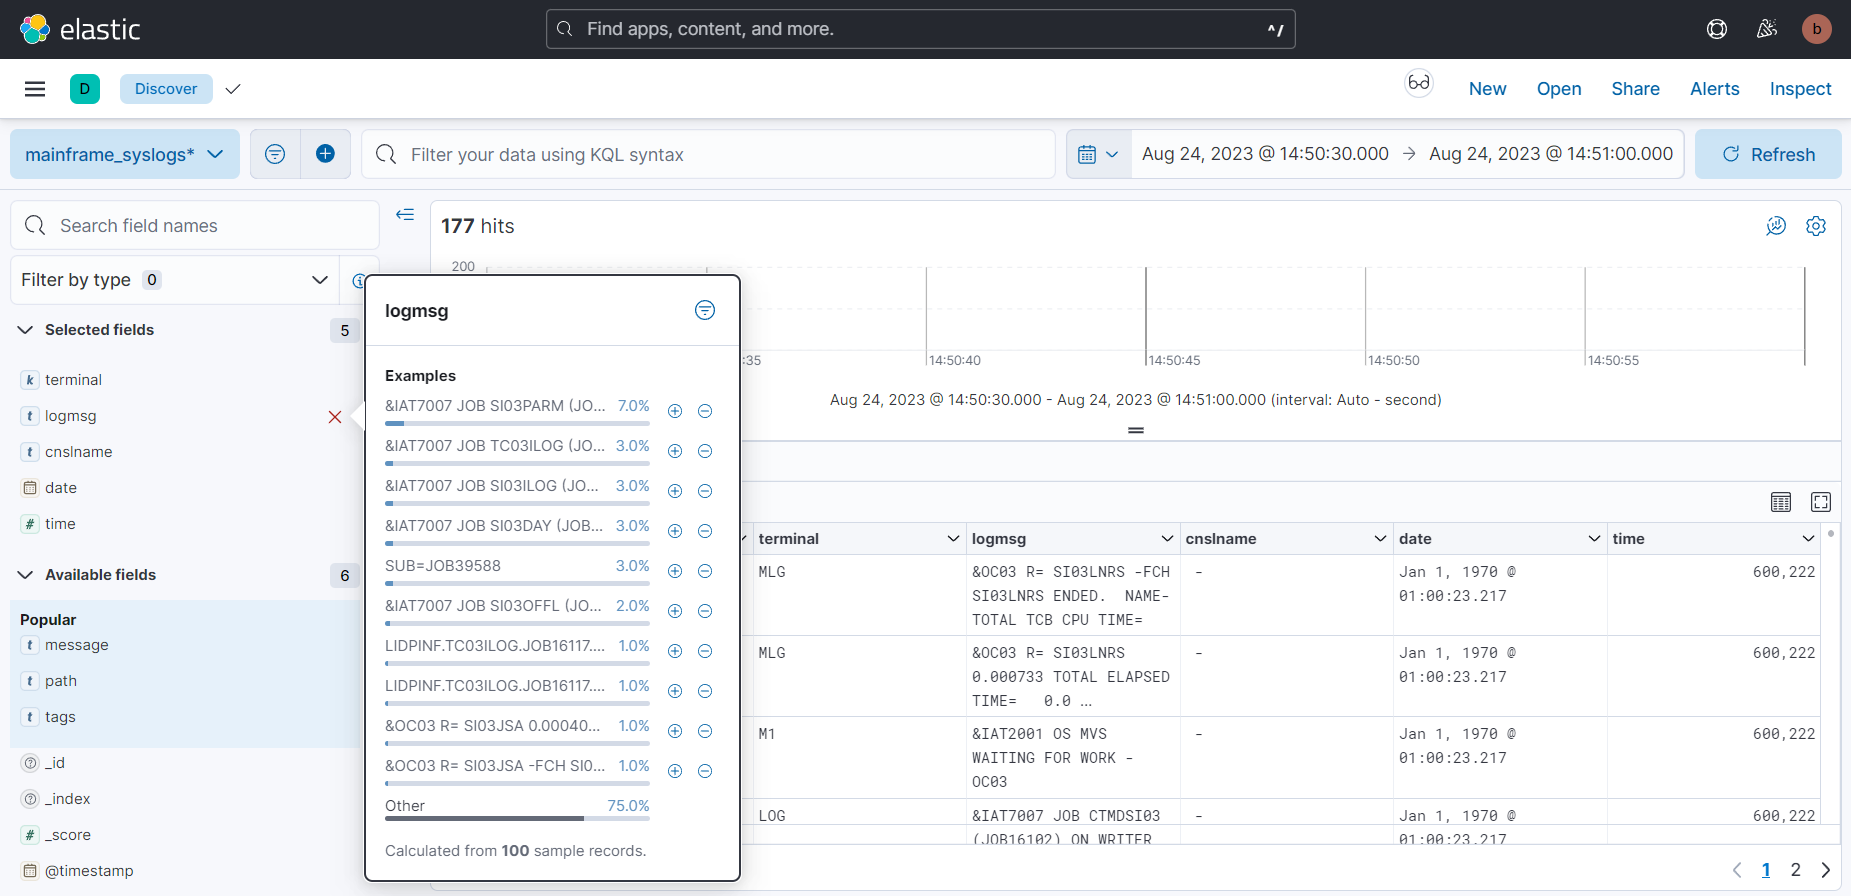
\includegraphics[width=0.50\linewidth]{bachproef//graphics/Kibana_stats_1.png}
    \caption{Statistieken 1}
    \label{fig:Statistieken 1}
\end{figure}

\begin{figure}[h]
    \centering
    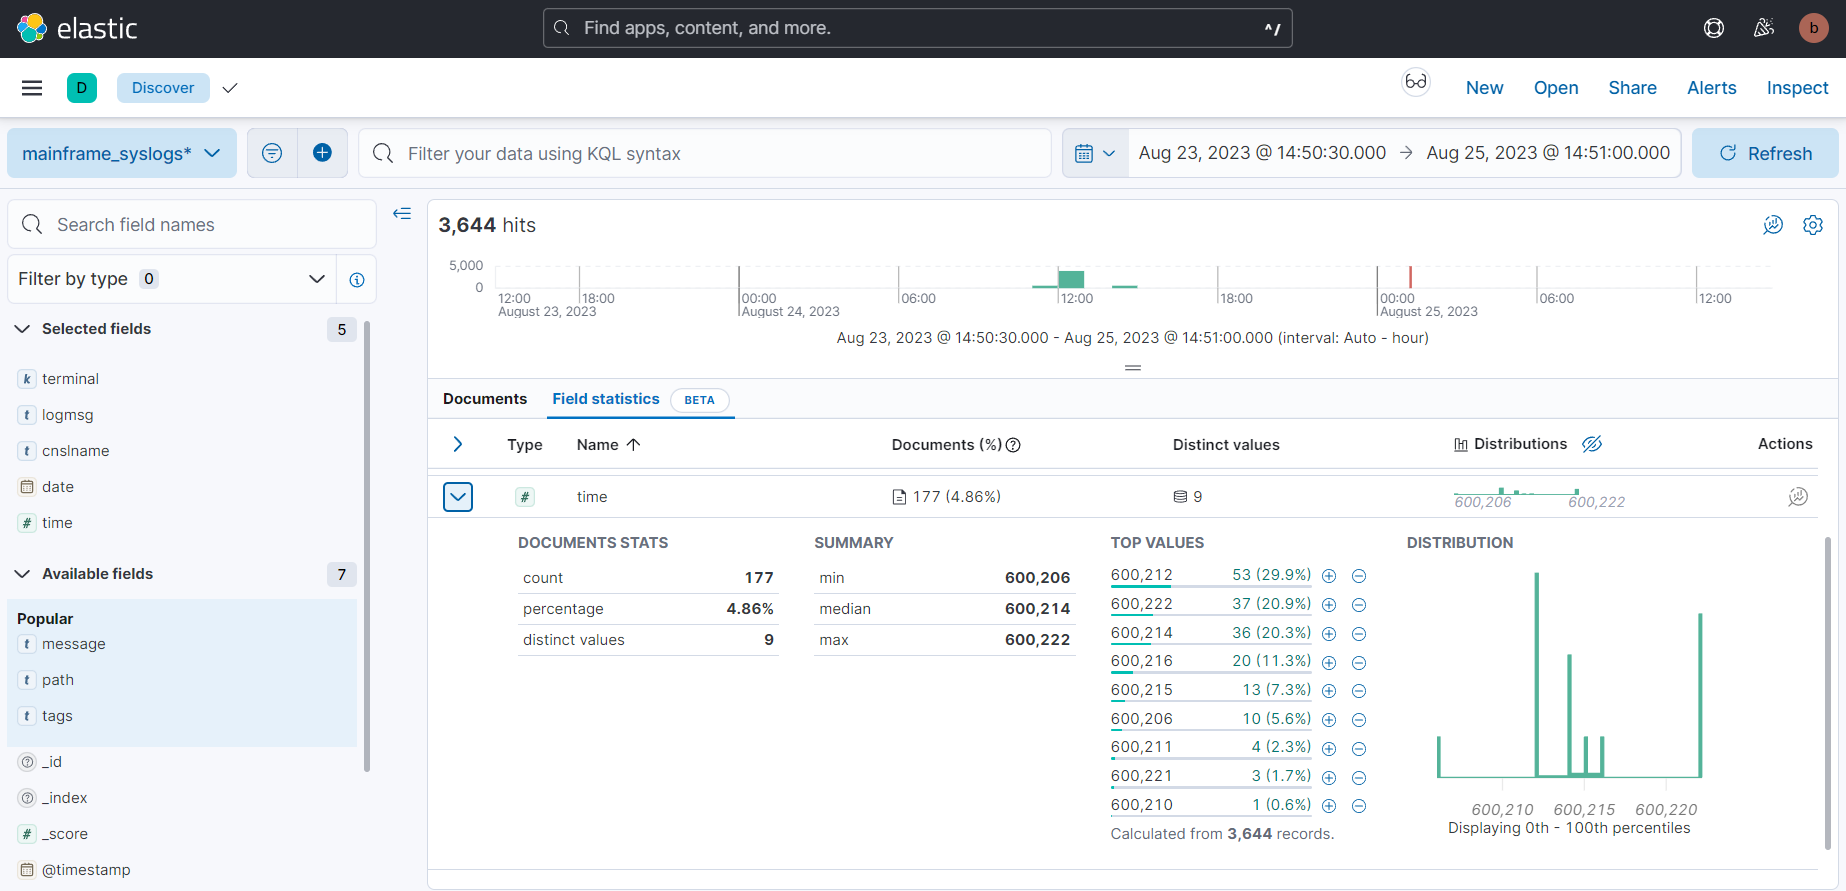
\includegraphics[width=0.50\linewidth]{Kibana_stats_2.png}
    \caption{Statistieken 2}
    \label{fig:Statistieken 2}
\end{figure}
\clearpage
\subsubsection{Paneel vier}
Dit paneel is bedoeld om het meest recente log te kunnen bekijken. Deze optie was al beschikbaar bij het openen van "Mainframe systemlogs." Alleen moesten de gewenste velden en datum worden geselecteerd. Bovendien kan dit eenvoudig worden gefilterd om relevante gegevens te bekijken.

\begin{figure}[h]
    \centering
    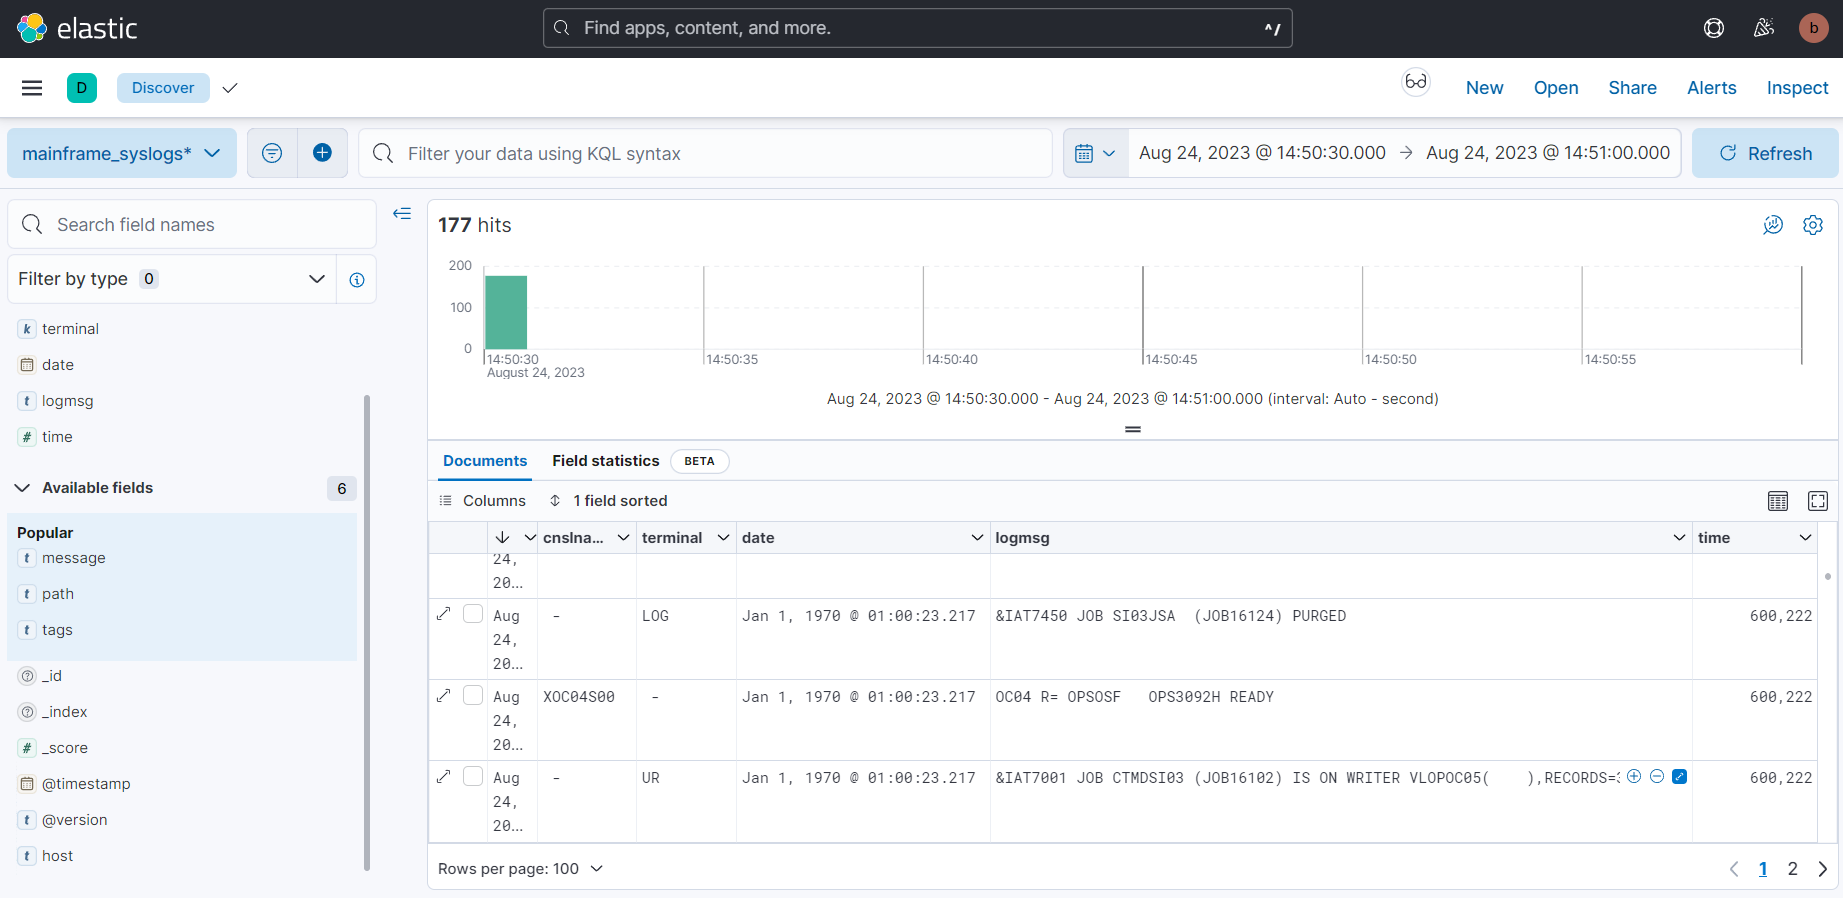
\includegraphics[width=0.50\linewidth]{Kibana_recent_log.png}
    \caption{De meest recente log}
    \label{fig:De meest recente log}
\end{figure}

\subsubsection{Paneel vijf}
Paneel 5 van de mockup is een basis tekstpaneel. Voor dit paneel is geen extra werk nodig.

\subsection{Kibana-dashboard}
Hoewel er geen dashboard is gemaakt, kan worden geconcludeerd uit de eerdere tests dat het mogelijk is om de mockup nauwkeurig te repliceren in Kibana. Hierdoor kan de mockup worden gebruikt als een nauwkeurige representatie voor de conclusies. Al deze panelen waren zeer eenvoudig te maken door op "create visualisation" te klikken, zoals weergegeven in de rechterbovenhoek van figuur 5.3. Daarna was het een kwestie van testen welke velden het beste werkten met welke visualisaties. Het is veilig om te concluderen dat het niet veel extra werk zou zijn geweest om deze visualisaties op te nemen in een dashboard.



%%=============================================================================
%% Conclusie
%%=============================================================================

\chapter{Conclusie}%
\label{ch:conclusie}

\section{Conclusie}
\begin{itemize}
    \item Kan een lid van het MFPOSS aan de hand van ELK makkelijker zien of er een abnormaliteit is in de systeem logs?
    \item Kan dit gebeuren op een manier waar MFPOSS niet te veel mankracht moet steken in het uitbreiden/behouden van het dashboard?
    \item Voldoet ELK aan de verwachtingen van MFPOSS?
\end{itemize}

Dit waren de onderzoeksvragen waarmee deze bachelorproef gestart is. Op de eerste twee vragen kan er positief geantwoorden. Desondanks dat er geen dashboard gemaakt is geweest en er eich een aantal problemen voordeden, blijkt het uit testen dat op Kibana uitgevoerd zijn geweest, dat het niet alleen simpel is om ermee te werken maar dat het ook een meerwaarde heeft. Dit betekent niet dat het waard is voor MFPOSS om te blijfven werken met ELK. Daarvoor moet er gekeken worden naar de vooropgezette MoSCow.

\subsection{Must have}
De 'Must Have' dat MFPOSS had opgesteld was dat er te zien valt of er berichten in voorkomen dat opmerkkelijk veel of weinig in de logs voorkomen. Dit is mogelijk met Kibana al is er geen deviatie detectie. Dat maakt het wel aanzienlijk moeilijker maar het is een verbetering dan tegenover manueel de logs te analyseren.ELK voldoet aan de 'Must haves' maar dit zou beter kunnen. Nu kan de vraag gesteld worden wat als Colruyt Group wel aan deviatie detectie zou doen, Wat voor impact zou dat dan hebben op de mogelijkheden om logs te analyseren? Dit is voor toekomstig onderzoek vatbaar.

\subsection{Should have}
De 'should haves' dat waren opgesteld waren dat het dashboard eenvoudig aanpasbaar moest zijn. Elke visualisatie optie dat is uitgestest geweest was makkelijk te maken. Een stap we niet hebben kunnen testen was het opslaan van een visualisatie naar een dashboard. Maar dit gaat niet veel extra werk meer opleveren aan MFPOSS. Deze voorwaarde is dus voldaan. Daarentegen weet men al dat deviatie detectie niet kan wat betkent dat deze vorwaarde onvoldaan is.  

\subsection{Could have}
Door het feit dat deviatie detectie niet wordt gedaan is het automatish doorsturen van een melding quasie onmogelijk om te doen. Zeker zonder daar te veel mankracht op te zetten. ELK voldoet dus niet and de 'Could haves'. Dit is aanzich geen probleem maar het blijft wel een minpunt. 

\subsection{Won't have}
ELK voldoet aan de 'Won't haves' door het simpel te houden en de mogelijkheid te hebben om zonder te veel werk zaken aan te passen of toe te voegen.

In conclusie voldoet de dashboard aan de verwachtingen van MFPOSS om logs te kunnen analyseren. Maar een groot minpunt is hier dat deviatie detectie geen optie was een belangrijk punt was voor hun. Het is nog steeds makkelijker om afwijkingen te zien op Kibana dan manueel in de logs. Er moet nog aan de integratie gesleuteld worden maar aangezien er twee teams op aan het werken zijn is extra werkbelast maar klein. Het is het dus waard voor MFPOSS om de logs over te zetten en een dashboard te maken. Dat geldt ook voor de mainframe teams dat aan het denken zijn om ELK te gebruiken in de toekomst. Het advies dat meegegeven wordt met MFPOSS is als volgt: Elk is de moeite waard en zeker als er een conversatie gestart wordt in verband met de deviatie detectie. Aangezien dit een groot aanwinst zou kunnen zijn. Maar de pluspunten zijn net meer als de minpunten. Als er zich nog te veel fouten blijven voordoen is dit een project dat even in hiatus zou moeten gaan tot dat er dringend vraag naar is.


\clearpage
\input{bachproef.bib}
%---------- Bijlagen -----------------------------------------------------------

\appendix

\chapter{Onderzoeksvoorstel}

Het onderwerp van deze bachelorproef is gebaseerd op een onderzoeksvoorstel dat vooraf werd beoordeeld door de promotor. Het onderwerp is met toestemming veranderd geweest naar het analyseren van mainfame systeemlogs. Dit is ook een bachelorproef in examenpeiode drie. Er is geen bachelorproef ingedient geweest in examenperiode één dus alles is nieuw.

%% TODO: 
%\section*{Samenvatting}

% Kopieer en plak hier de samenvatting (abstract) van je onderzoeksvoorstel.

% Verwijzing naar het bestand met de inhoud van het onderzoeksvoorstel
%---------- Inleiding ---------------------------------------------------------

\section{Introductie}%
\label{sec:introductie}

In hun kern zijn mainframes eigenlijk computers met een grote hoeveelheid geheugen en data processoren. Daarmee kan het een kolossaal hoeveelheid aan bewerkingen uitvoeren en gegevens verwerken. Dit doet het mainframe op een zeer betrouwbare, veilige en schaalbare manier. Voor het mainframe zijn deze 3 concepten erg van belang en blinkt het er ook meteen in uit. Een bedrijf zou van hun mainframe minstens 99.999 of '\textit{5 nines}' beschikbaarheid mogen verwachten dat betekent dat per jaar een mainframe niet meer als 5.26 minuten onverwacht niet beschikbaar is. Het is zelfs niet ongehoord dat een mainframe jaren aan een stuk draait zonder één moment waar het onverwachts onbeschikbaar is. Dit is tot op het punt gekomen waar dat voor IBM's zSystems de z voor "zero downtime" staat. Het is dus niet moeilijk om te concluderen dat betrouwbaarheid zeer hoog staat voor mainframes. Er zijn natuurlijk nog meer redenen waarom het mainframe een belangrijk platform is. Maar het is vooral door het uitblinken in deze 3 concepten dat het een cruciaal deel van onze samenleving is geworden. Banken, Overheden, Vliegtuigmaatschappijen en nog veel meer steunen op deze concepten om alles vlot en veilig te laten verlopen en dit met zo min mogelijk momenten van onbeschikbaarheden te hebben. Het is dus belangrijk om deze concepten te her-evalueren en verbeteren waar mogelijk zodat het platform alsmaar blijft evolueren met de tijden. Colruyt Group ziet op dit moment wel een plaats waar er mogelijks verbetering in kan. Om ervoor te zorgen dat hun systeem blijft draaien op een optimale wijzen hebben ze systeem logs. Het probleem daarbij is dat die logs miljoenen rijen lang kunnen zijn en voor een mens is het quasi onmogelijk om met zekerheid te bevestigen of dat er geen afwijking is gebeurd van het normaal verloop. Hier komen log analyzers zoals ELK en DataDog bij kijken. Log analyzers worden nu volop gebruikt door traditionele platformen om logs te analyseren en te visualiseren met grafieken van hoge kwaliteit. Er kunnen veel positieve zaken over gehoord worden maar kunnen dezelfde praktijken en tools gebruikt worden voor de mainframe logs?


%---------- Stand van zaken ---------------------------------------------------

\section{State-of-the-art}%
\label{sec:state-of-the-art}

\subsection{Mainframe?}
Een mainframe is zoals eerder besproken een computer die gemaakt is om vlot en veilig transacties te kunnen uitvoeren. Er is hier een nadruk op veiligheid en betrouwbaarheid. Logs maken daar een groot deel van. Zonder logs kan men niet weten of het systeem goed aan het draaien is of niet en daarom is er een extensieve log systeem voorzien. Het probleem is dat men die aanzienlijk groot is. Men spreekt hier van miljoenen rijen en zelfs een ervaren werknemer zou hier makkelijk zaken kunnen missen. Dit is dus het probleem waar Colruyt Group vandaag een antwoord op zoekt. ~\autocite{IBM2023(1),IBM2023(2),IBMArchives}

\subsubsection{z/16}
z16 een mainframe gemaakt door IBM. Deze mainframe is in 2023 het meest recente beschikbare mainframe. Deze mainframe wordt gehanteerd in Colruyt en gaat op kleine mate beschikbaar worden gesteld voor dit onderzoek. \newline ~\autocite{Laura2023} 

\subsection{Log analysers}
In dit hoofdstuk gaan een paar van de meest bekende analyzers kort besproken worden. Dit zijn dan ook de analyzers dat onderzocht gaan worden. De keuzes werden gemaakt op basis van beschikbaarheid, aanbevelingen en poteniele meerwaarde aan Colruyt Group. Enige verdere studies dat andere log analyzers zouden gebruiken zouden hun werk kunnen baseren en vergelijken met deze analyzers. Aangezien in de wereld van software alles snel beweegt zou er wel moeten uitgekeken worden naar mogelijke nieuwe updates. Bij elke besproken log analyzer gaat er een versienummer vermeld worden. 

\subsubsection{ELK of Elastic stack}
Versie: 8.10.3 \newline
ELK is een groep van voormalige open-source softwareapplicaties dat samenwerken om de ELK-stack te vormen. Er zijn drie hoofdapplicaties dat een ELK-stack maken en die zijn Elasticsearch, Logstash en Kibana. Daarbij komen soms andere applicaties zoals Beats ook bij kijken. Gemaakt en beheerd door Elastic, ELK dient om logs te analyseren en te visualiseren. Zo kunnen teams niet alleen hun logs overzichtelijk bekijken maar ook grafieken maken en vergelijken met vorige logs. ~\autocite{Elatic(1),DotanHorovits}

\begin{itemize}
    \item Elasticsearch is een prominente \newline NoSQL database gebouwd op de krachtige Lucene zoekmachine, bekend om zijn \newline robuuste mogelijkheden op het gebied van gegevensopslag en -opvraging. ELk is een zoekserver is geschreven in Java en het blinkt uit in het indexeren van heterogene gegevenstypen.~\autocite{GedalBer}
    \item Logstash is een gegevensverwerkingstool die oorspronkelijk is ontworpen voor log-analyse, maar zich heeft ontwikkeld tot een veelzijdige gegevensverwerkingstool. Het werkt als een pijpleiding in 3 fases: invoer, filter en uitvoer. ~\autocite{Jamie2017,JugensToit}
    \item Kibana zorgt voor de visualisatie van de data. Dit aan de hand van een dashboard met grafieken, kaarten, cijfers of tekst.~\autocite{DavidTaylor2}
    \item Beats is een applicatie dat vaak ook wordt gebruikt in een elastic stack doordat het de logs naar ELK krijgen vereenvoudigd. \newline ~\autocite{objectrocket}
\end{itemize}

\subsubsection{Grafana Loki}
Versie: v2.9.x \newline
Grafana is een open source data\newline -visualisatieplatform. Het is gemaakt en onderhouden door Grafana Labs. Met Grafana kunnen gebruikers hun gegevens bekijken via grafieken en diagrammen die zijn samengevoegd in een dashboard. Dit is gelijkaardig aan de meeste log analyzers. Dit komt omdat dashboarden zorgen voor een makkelijkere interpretatie en begrip van de data. Op grafana kunt ook waarschuwingen instellen voor uw informatie en metingen. Dit zorgt ervoor dat u sneller kan inspringen bij geval van problemen. Grafana is gebouwd op open principes en het geloof dat gegevens toegankelijk moeten zijn voor de hele organisatie en niet alleen voor een kleine groep mensen. \autocite{RedHat2022,Grigor2023}

\subsubsection{DataDog}
Versie: 7 \newline
Datadog is de derde monitoring- en analysetool dat we bespreken. Het kan prestatiegegevens en gebeurtenisbewaking bieden voor infrastructuur en Cloud services. Waaronder servers en databases. Het is beschikbaar voor implementatie op locatie of als een SaaS-oplossing en ondersteunt diverse besturingssystemen en Cloud serviceproviders. Datadog gebruikt een Go-agent en heeft integraties met verschillende diensten en tools. Het biedt aanpasbare dashboards en meldingen voor prestatieproblemen via verschillende communicatie platformen. \autocite{DataDog2021}

\subsection{Linux}
Linux is een gratis open source besturingssysteem. Dit betekent dat iedereen dat interesse heeft Linux kan bestuderen en zelf aanpassen naar eigen mate en zelf distribueren naar anderen. Door deze vrijheid en andere voordelen is Linux één van 's werelds grootse besturingssystemen geworden. Waarom Linux een rol speelt in dit onderzoekt wordt verder besproken in hoofdstuk 3 "Methodologie". \autocite{RedHat2023}
%---------- Methodologie ------------------------------------------------------
\section{Methodologie}%
\label{sec:methodologie}
Aangezien er in dit onderzoek een vergelijking gaat gemaakt worden uit drie verschillende applicaties is het verstandig om ook criteria op te stellen. Die criteria gaan overlegd worden met Colruyt Group IT en enig mogelijkse toekomstige onderzoeken zullen deze criteria eerst moeten revalueren en aanpassen naar eigen voorkeur. De criteria kunnen in een MoSCoW-formaat gemaakt en gebruikt worden. Vervolgens gaan er prototypes moeten opgesteld worden van elke analyzer. Eén prototype per applicatie is voldoende, al zouden meerdere natuurlijk ideaal zijn. Colruyt Group zal een test Linux server aanbieden waarop de analyzers mogen geïnstalleerd worden. De Linux server loopt op het mainframe maar er wordt niet gepland om de analyzers rechtstreeks op de mainframe te zetten. Dit omdat er een grote zekerheid is dat het te moeilijk zou zijn. Terwijl dat op een Linux server beter gedocumenteerd en ondersteund is langs beide kanten. Eens de prototypes klaar zijn worden ze gemeten aan de hand van de criteria en kan er een gedetailleerde aanrading met prototype overgemaakt worden aan Colruyt Group IT.


%---------- Verwachte resultaten ----------------------------------------------
\section{Verwacht resultaat, conclusie}%
\label{sec:verwachte_resultaten}
Het optimale resultaat van dit onderzoek zouden meerdere werkende prototypes zijn met één uitblinker dat kan aangeraden worden aan Colruyt Group It. Natuurlijk is er een mogelijkheid dat er een analyzer niet compatibel is met de omgeving dat we opzetten maar in het slechtste geval zou minstens één analyzer moeten werken en een vervanging gezocht moeten worden om toch een vergelijking te kunnen doen met twee werkende prototypes.




%%---------- Andere bijlagen --------------------------------------------------
% TODO: Voeg hier eventuele andere bijlagen toe. Bv. als je deze BP voor de
% tweede keer indient, een overzicht van de verbeteringen t.o.v. het origineel.
%\input{...}

%%---------- Backmatter, referentielijst ---------------------------------------

\backmatter{}

\setlength\bibitemsep{2pt} %% Add Some space between the bibliograpy entries
\printbibliography[heading=bibintoc]

\end{document}
